\chapter{Dopamine in reinforcement learning}


\section{Decision making}

\begin{description}
    \item[Decision-making] \marginnote{Decision-making}
        Voluntary process that leads to the selection of an action based on sensory information.

        Decisions are inherently non-deterministic as:
        \begin{itemize}
            \item Agents make inconsistent choices.
            \item Agents make choices unaware of the full consequences (uncertainty).
            \item Internal and external signals are noisy.
        \end{itemize}

        \begin{remark}
            From an evolutionary point of view, stochasticity in decisions increases the chances of survival.
        \end{remark}

        \begin{remark}
            Decision-making studied within the neuroscience field is actually studying cognition.
            It involves studying the neural processes underlying a variety of mental functions.
        \end{remark}
    

    \item[Perceptual decision-making] \marginnote{Perceptual decision-making}
        An agent selects between action $A$ and $B$ based on weak or noisy external signals (e.g. ``do you see $A$ or $B$?'').

        In this case, uncertainty comes from the external stimulus.

        \begin{figure}[H]
            \centering
            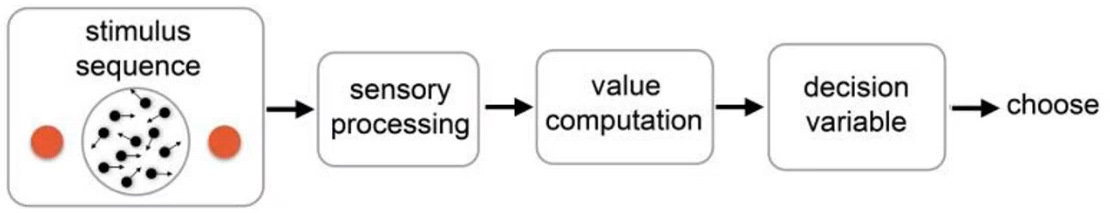
\includegraphics[width=0.55\linewidth]{./img/perceptual_dm.png}
        \end{figure}

    \item[Value-based decision-making] \marginnote{Value-based decision-making}
        An agent selects between action $A$ and $B$ based on its subjective preferences (e.g. ``do you prefer $A$ or $B$?'').

        In this case, uncertainty comes from the value associated with the action.

        \begin{figure}[H]
            \centering
            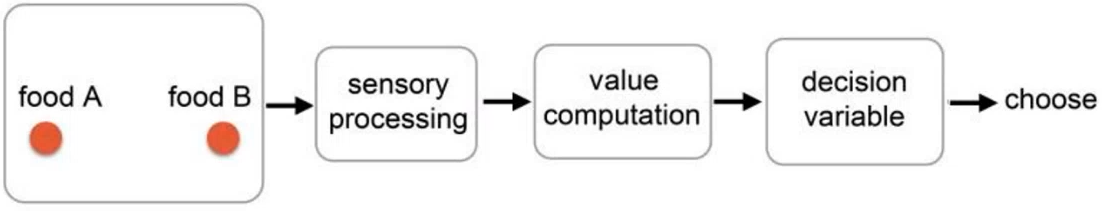
\includegraphics[width=0.55\linewidth]{./img/value_dm.png}
        \end{figure}

    
    \item[Decision-making processes]
        Decision-making involves the following processes:
        \begin{descriptionlist}
            \item[Representation] \marginnote{Representation}
                States, actions, and internal and external factors are identified.

            \item[Valuation] \marginnote{Valuation}
                A value is assigned to the possible alternatives.

            \item[Choice] \marginnote{Choice}
                Values are compared and a proper action is selected.

            \item[Outcome evaluation] \marginnote{Outcome evaluation}
                After performing the action, the desirability of the outcome is measured (reward prediction error).

            \item[Learning] \marginnote{Learning}
                Feedback signals are used to update the processes and improve the quality of future decisions.
        \end{descriptionlist}

        \begin{figure}[H]
            \centering
            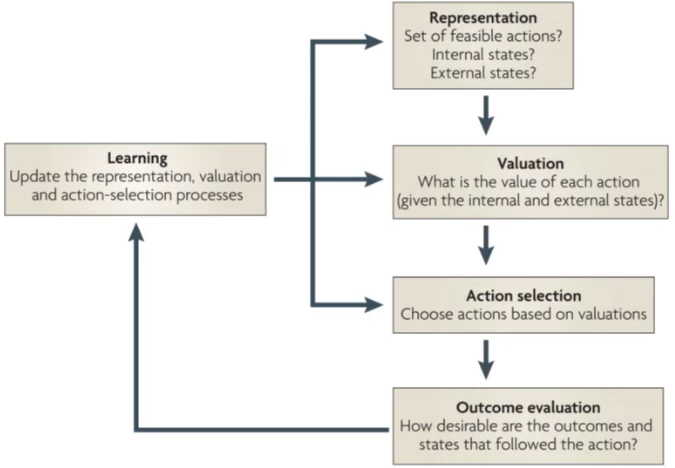
\includegraphics[width=0.55\linewidth]{./img/dm_processes.png}
        \end{figure}


    \item[Valuation circuitry] \marginnote{Valuation circuitry}
        Involves neurons sensitive to reward value.
        They are spread in the brain, both in the cortical and subcortical regions.

        \begin{figure}[H]
            \centering
            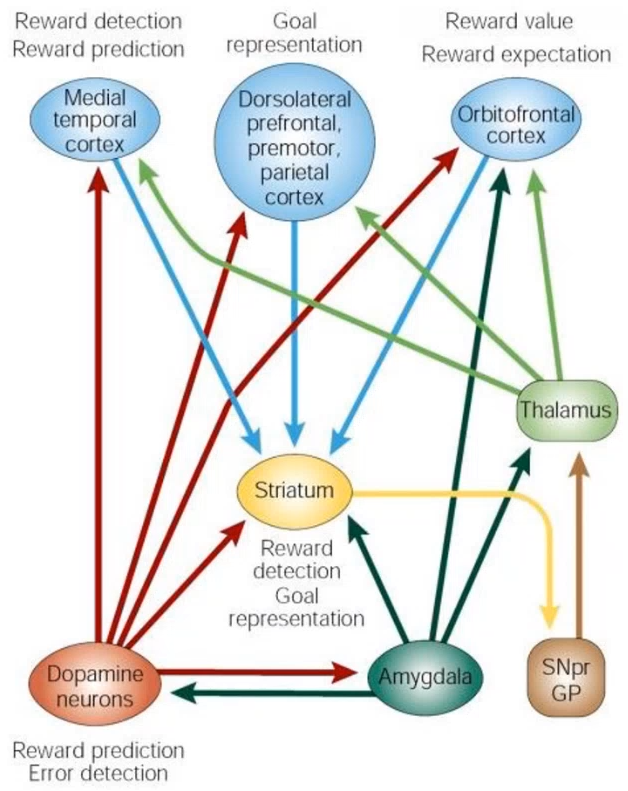
\includegraphics[width=0.38\linewidth]{./img/valuation_circuitry.png}
        \end{figure}

        
    \item[Decision-making theories] \marginnote{Decision-making theories}
        \begin{descriptionlist}
            \item[Economic learning] \marginnote{Economic learning}
                Decision-making involving the selection of an action with the maximum utility.

            \item[Reinforcement learning] \marginnote{Reinforcement learning}
                Decision-making involving the probabilistic selection of an action.
        \end{descriptionlist}

        \begin{figure}[H]
            \centering
            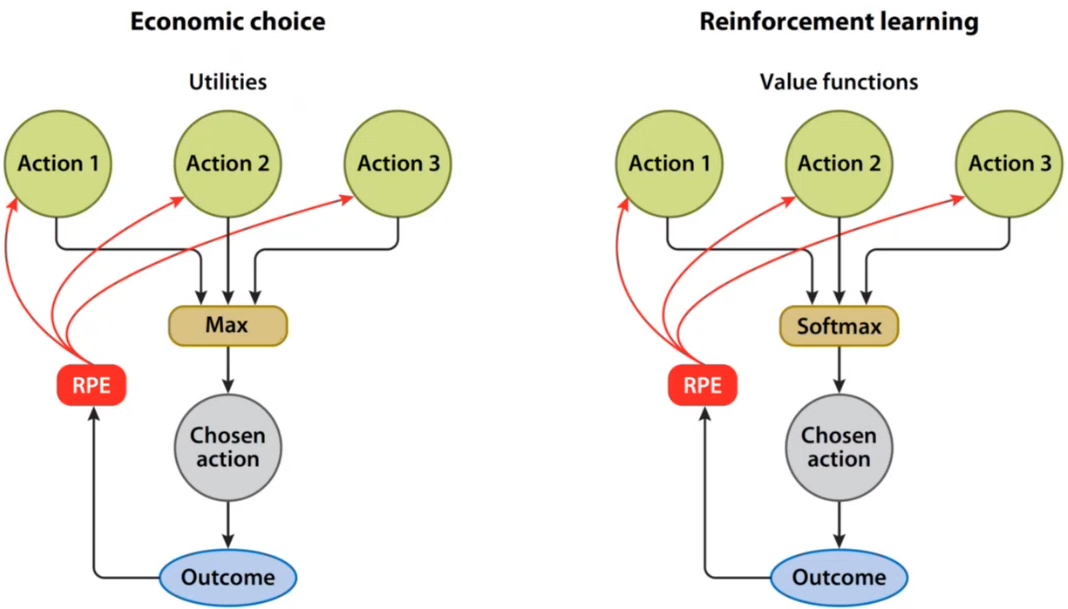
\includegraphics[width=0.55\linewidth]{./img/dm_theories.png}
        \end{figure}
\end{description}



\section{Reinforcement learning}

\begin{description}
    \item[Reinforcement learning (RL)] \marginnote{Reinforcement learning (RL)}
        Learn a mapping between states and actions aiming to maximize the expected cumulative future reward.

        \begin{description}
            \item[Markov conditional independence] At any time step, all future states and rewards only depend on the current state and action. 
        \end{description}


    \item[Bellman equation] \marginnote{Bellman equation}
        Given an action $a_t$ performed in the state $s_t$ following a policy $\pi$,
        the expected future reward is given by the following equation:
        \[ Q_\pi(s_t, a_t) = r_t + \gamma \sum_{s_{t+1}} \prob{s_{t+1 | s_t, a_t}} Q_\pi(s_{t+1}, \pi(s_{t+1})) \]
        where $\gamma$ is a discount factor.
\end{description}


\subsection{RL classes}

\begin{description}
    \item[Model-based] \marginnote{Model-based}
        Aims to learn the right-hand side of the Bellman equation.
        This requires knowing the state transition distribution $\mathcal{P}$ which is costly.

    \item[Model-free] \marginnote{Model-free}
        Aims to directly learn the left-hand side of the Bellman equation by estimating $Q_\pi$ from experience.
        Agents use states, actions and rewards they experienced by averaging them to update a table of long-run reward predictions that
        approximate the right-hand side of the Bellman equation.

        \begin{description}
            \item[Temporal difference learning] \marginnote{Temporal difference learning}
                The reward prediction error at time $t$ is obtained by comparing the expected reward at time $t$ and at the next time step $t+1$:
                \[ \delta_t = r_t + \gamma Q(s_{t+1}, a_{t+1}) - Q(s_t, a_t) \]
        \end{description}
\end{description}

\begin{example}[Rat in maze]
    A rat has to navigate a maze with two crossroads and two different outcomes.
    \begin{figure}[H]
        \centering
        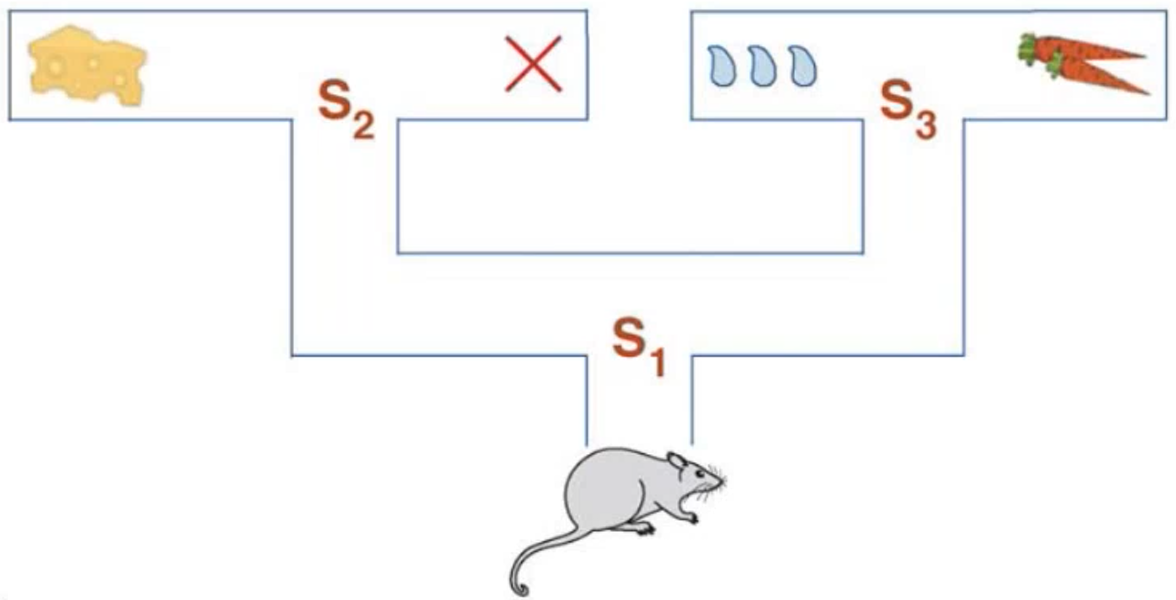
\includegraphics[width=0.4\linewidth]{./img/rat_maze1.png}
    \end{figure}

    Two strategies can be developed:
    \begin{descriptionlist}
        \item[Model-based]
            By learning the model of the environment, the rat can decide its path by using a search tree.
            The path can be changed depending on its motivational state (e.g. hungry or thirsty) showing a goal-directed behavior.

        \item[Model-free] 
            The value of each state-action pair is stored and action selection consists of choosing the highest cached value at the current state.
            Values do not consider the identity of the outcome and are therefore decoupled from the motivational state of the animal.

            Nevertheless, if the motivational state is stored as part of the environmental state, the animal would be able to account for it.
    \end{descriptionlist}

    \begin{figure}[H]
        \centering
        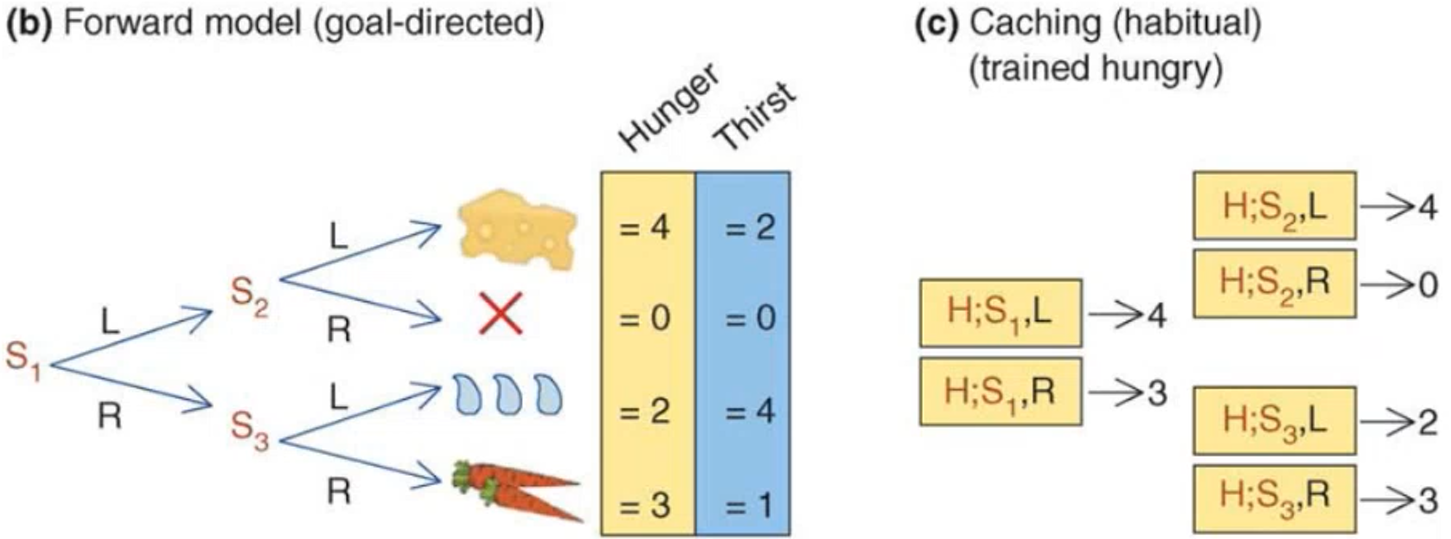
\includegraphics[width=0.6\linewidth]{./img/rat_maze2.png}
    \end{figure}
\end{example}



\section{Dopaminergic system}

There is strong evidence showing that the dopaminergic system is highly involved in reinforcement learning 
for predicting both natural rewards and addictive drugs.

\begin{description}
    \item[Dopamine pathways] \marginnote{Dopamine pathways}
        Dopamine projections include:
        \begin{descriptionlist}
            \item[Nigrostriatal system] Mostly associated with motor functions (action policy).
            \item[Meso-cortico-limbic system] Mostly associated with motivation (value function).
        \end{descriptionlist}

        \begin{figure}[H]
            \centering
            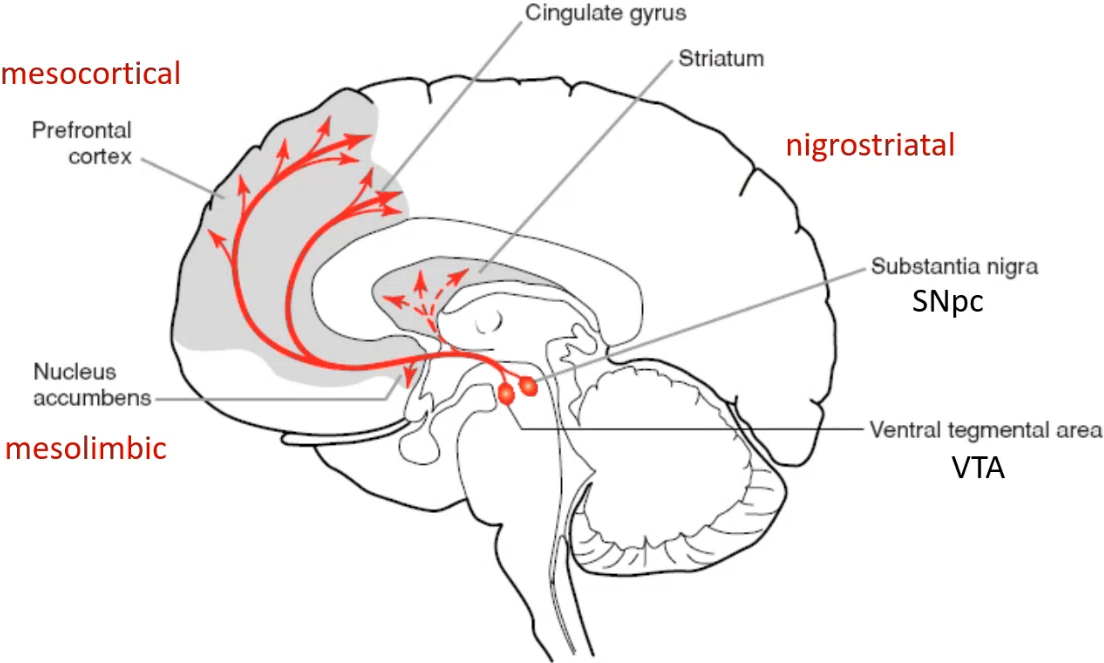
\includegraphics[width=0.5\linewidth]{./img/dopamine_pathways.png}
        \end{figure}

    \item[Actor/critic architecture] \marginnote{Actor/critic architecture}
        Model with two components:
        \begin{descriptionlist}
            \item[Critic]
                Takes as input a state and is responsible for learning and storing state values.
                It also receives the reward from the environment and 
                computes, through a temporal difference module, 
                the prediction error $\delta_t$ that is used to update its own state values and train the actor.

            \item[Actor] 
                Takes as input a state and maps it to an action policy $\pi(a, s)$ that is used to determine the action to perform.
        \end{descriptionlist}

        \begin{figure}[H]
            \centering
            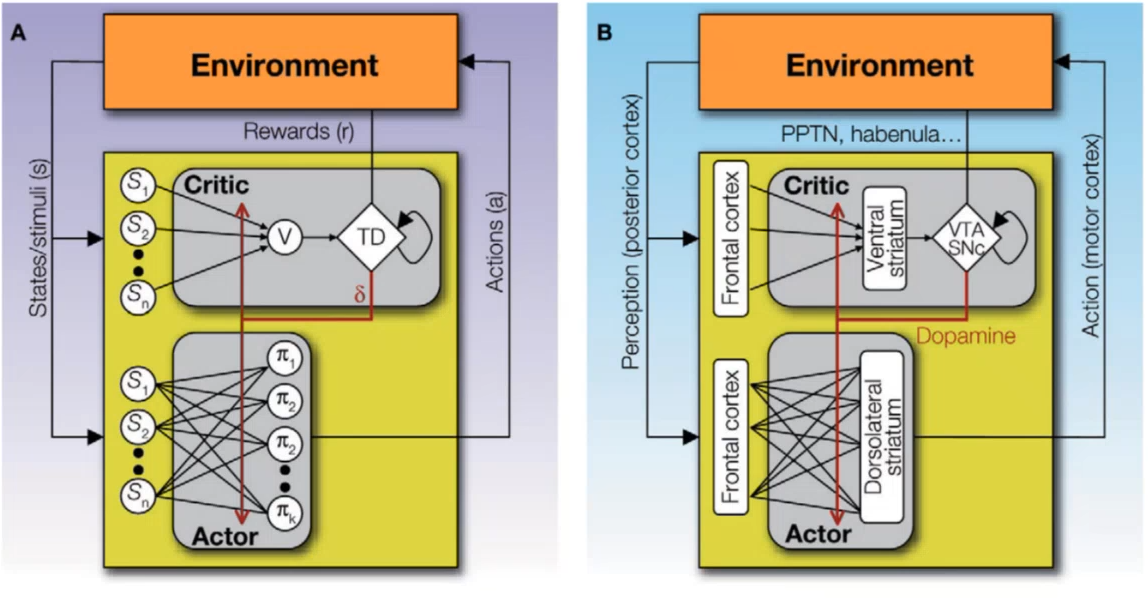
\includegraphics[width=0.65\linewidth]{./img/actor_critic.png}
            \caption{
                \parbox[t]{0.6\linewidth}{
                    Actor/critic architecture (A) and a possible mapping of the architecture onto neural substrates (B)
                }
            }
        \end{figure}
\end{description}


\begin{description}
    \item[Dopamine properties]
        \phantom{}

        \begin{description}
            \item[Phasic response] \marginnote{Dopamine phasic response}
                Depending on the stimulus, dopamine neurons can show excitatory or inhibitory responses.
                This can be interpreted as a reward prediction error.

                \begin{remark}
                    About 75\% of dopamine neurons are activated when there is a rewarding stimulus
                    and about 14\% of dopamine neurons are activated in response to an aversive stimulus.
                \end{remark}

                \begin{casestudy}[Dopamine as reward prediction error \cite{monkey_dopamine}]
                    A monkey is required to touch the content of a box for which it does not have vision.

                    It has been seen that dopamine neurons respond differently based on the content of the box.
                    This is consistent with the fact that dopamine is used as a prediction error signal.
                
                    \begin{figure}[H]
                        \centering
                        \begin{subfigure}{0.48\linewidth}
                            \centering
                            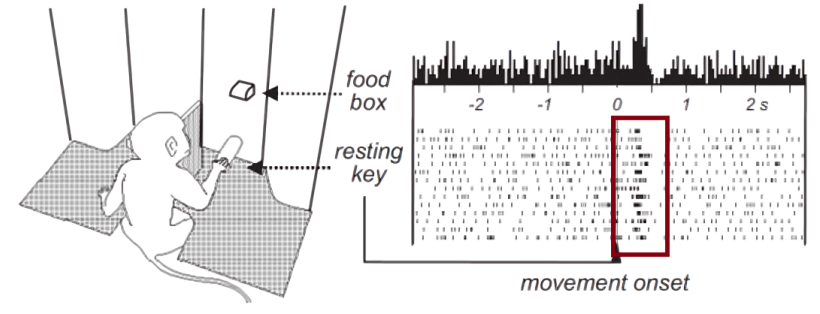
\includegraphics[width=0.9\linewidth]{../module1/img/dopamine_monkey1.png}
                        \end{subfigure}
                        \begin{subfigure}{0.48\linewidth}
                            \centering
                            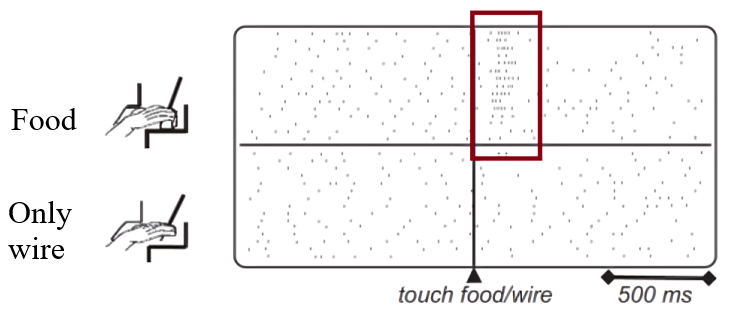
\includegraphics[width=0.9\linewidth]{../module1/img/dopamine_monkey2.png}
                        \end{subfigure}
                    \end{figure}
                \end{casestudy}
            

            \item[Bidirectional prediction] \marginnote{Dopamine bidirectional prediction}
                Dopamine captures both an improvement (positive prediction error) and a worsening (negative prediction error) of the reward.

                \begin{casestudy}[Dopamine bidirectional prediction error \cite{dopamine_bidirectional}]
                    It has been observed that the dopaminergic response differs depending on the amount of reward.

                    \begin{figure}[H]
                        \centering
                        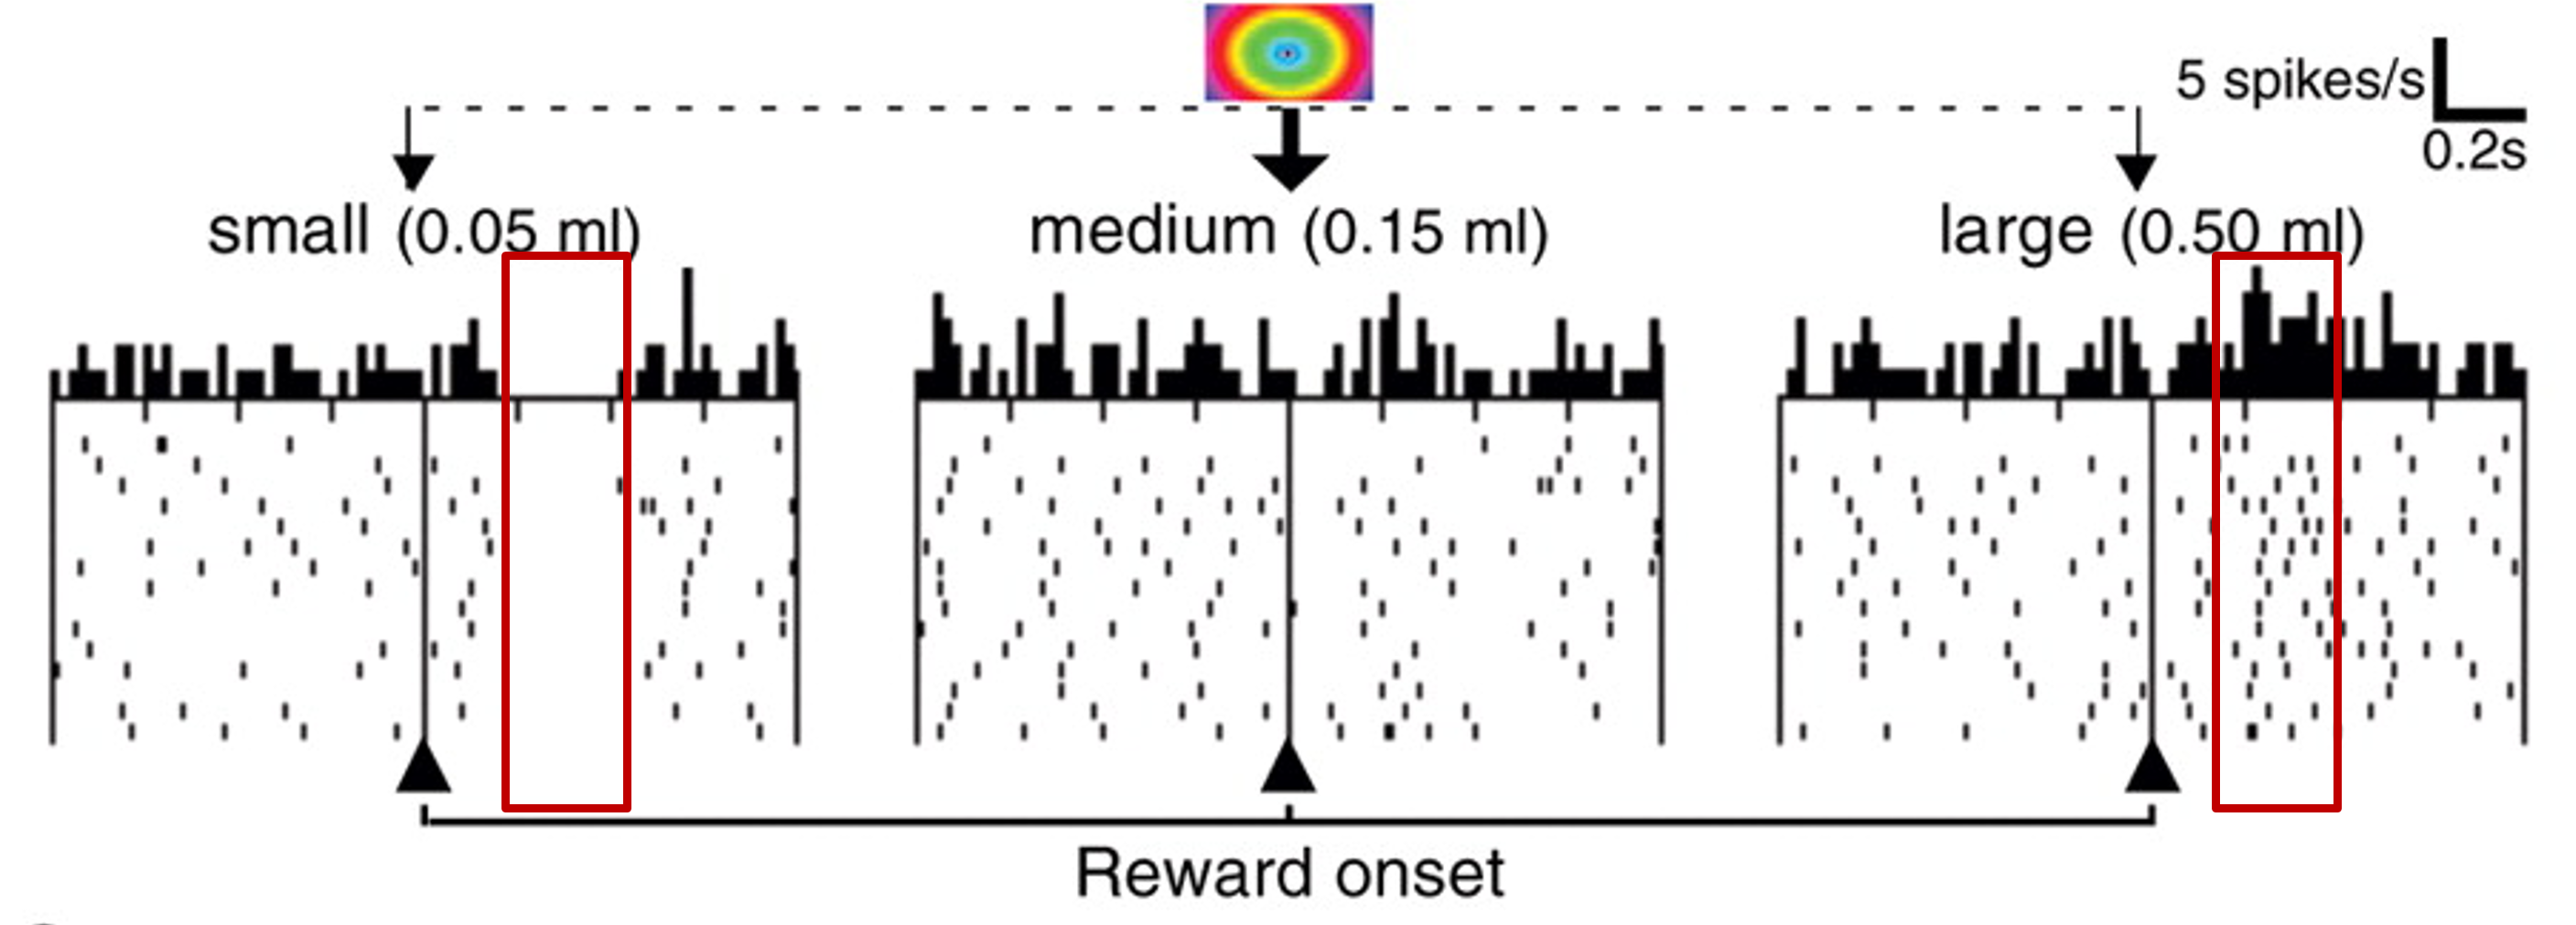
\includegraphics[width=0.65\linewidth]{../module1/img/dopamine_expected2.png}
                        \caption{
                            \parbox[t]{0.65\linewidth}{
                                Dopamine response of a monkey trained on a medium amount of reward
                            }
                        }
                    \end{figure}
                \end{casestudy}


            \item[Transfer] \marginnote{Dopamine transfer}
                Dopaminergic activity shifts from responding to the reward to responding to the conditioned stimulus that predicts it.

                \begin{casestudy}[Dopamine transfer \cite{dopamine_transfer, dopamine_transfer2}]
                    It has been seen that the dopaminergic response transfers from the moment of receiving the reward to the stimuli associated with it (CS).
                    This is in line with the temporal difference model. 

                    \begin{figure}[H]
                        \centering
                        \begin{subfigure}{0.48\linewidth}
                            \centering
                            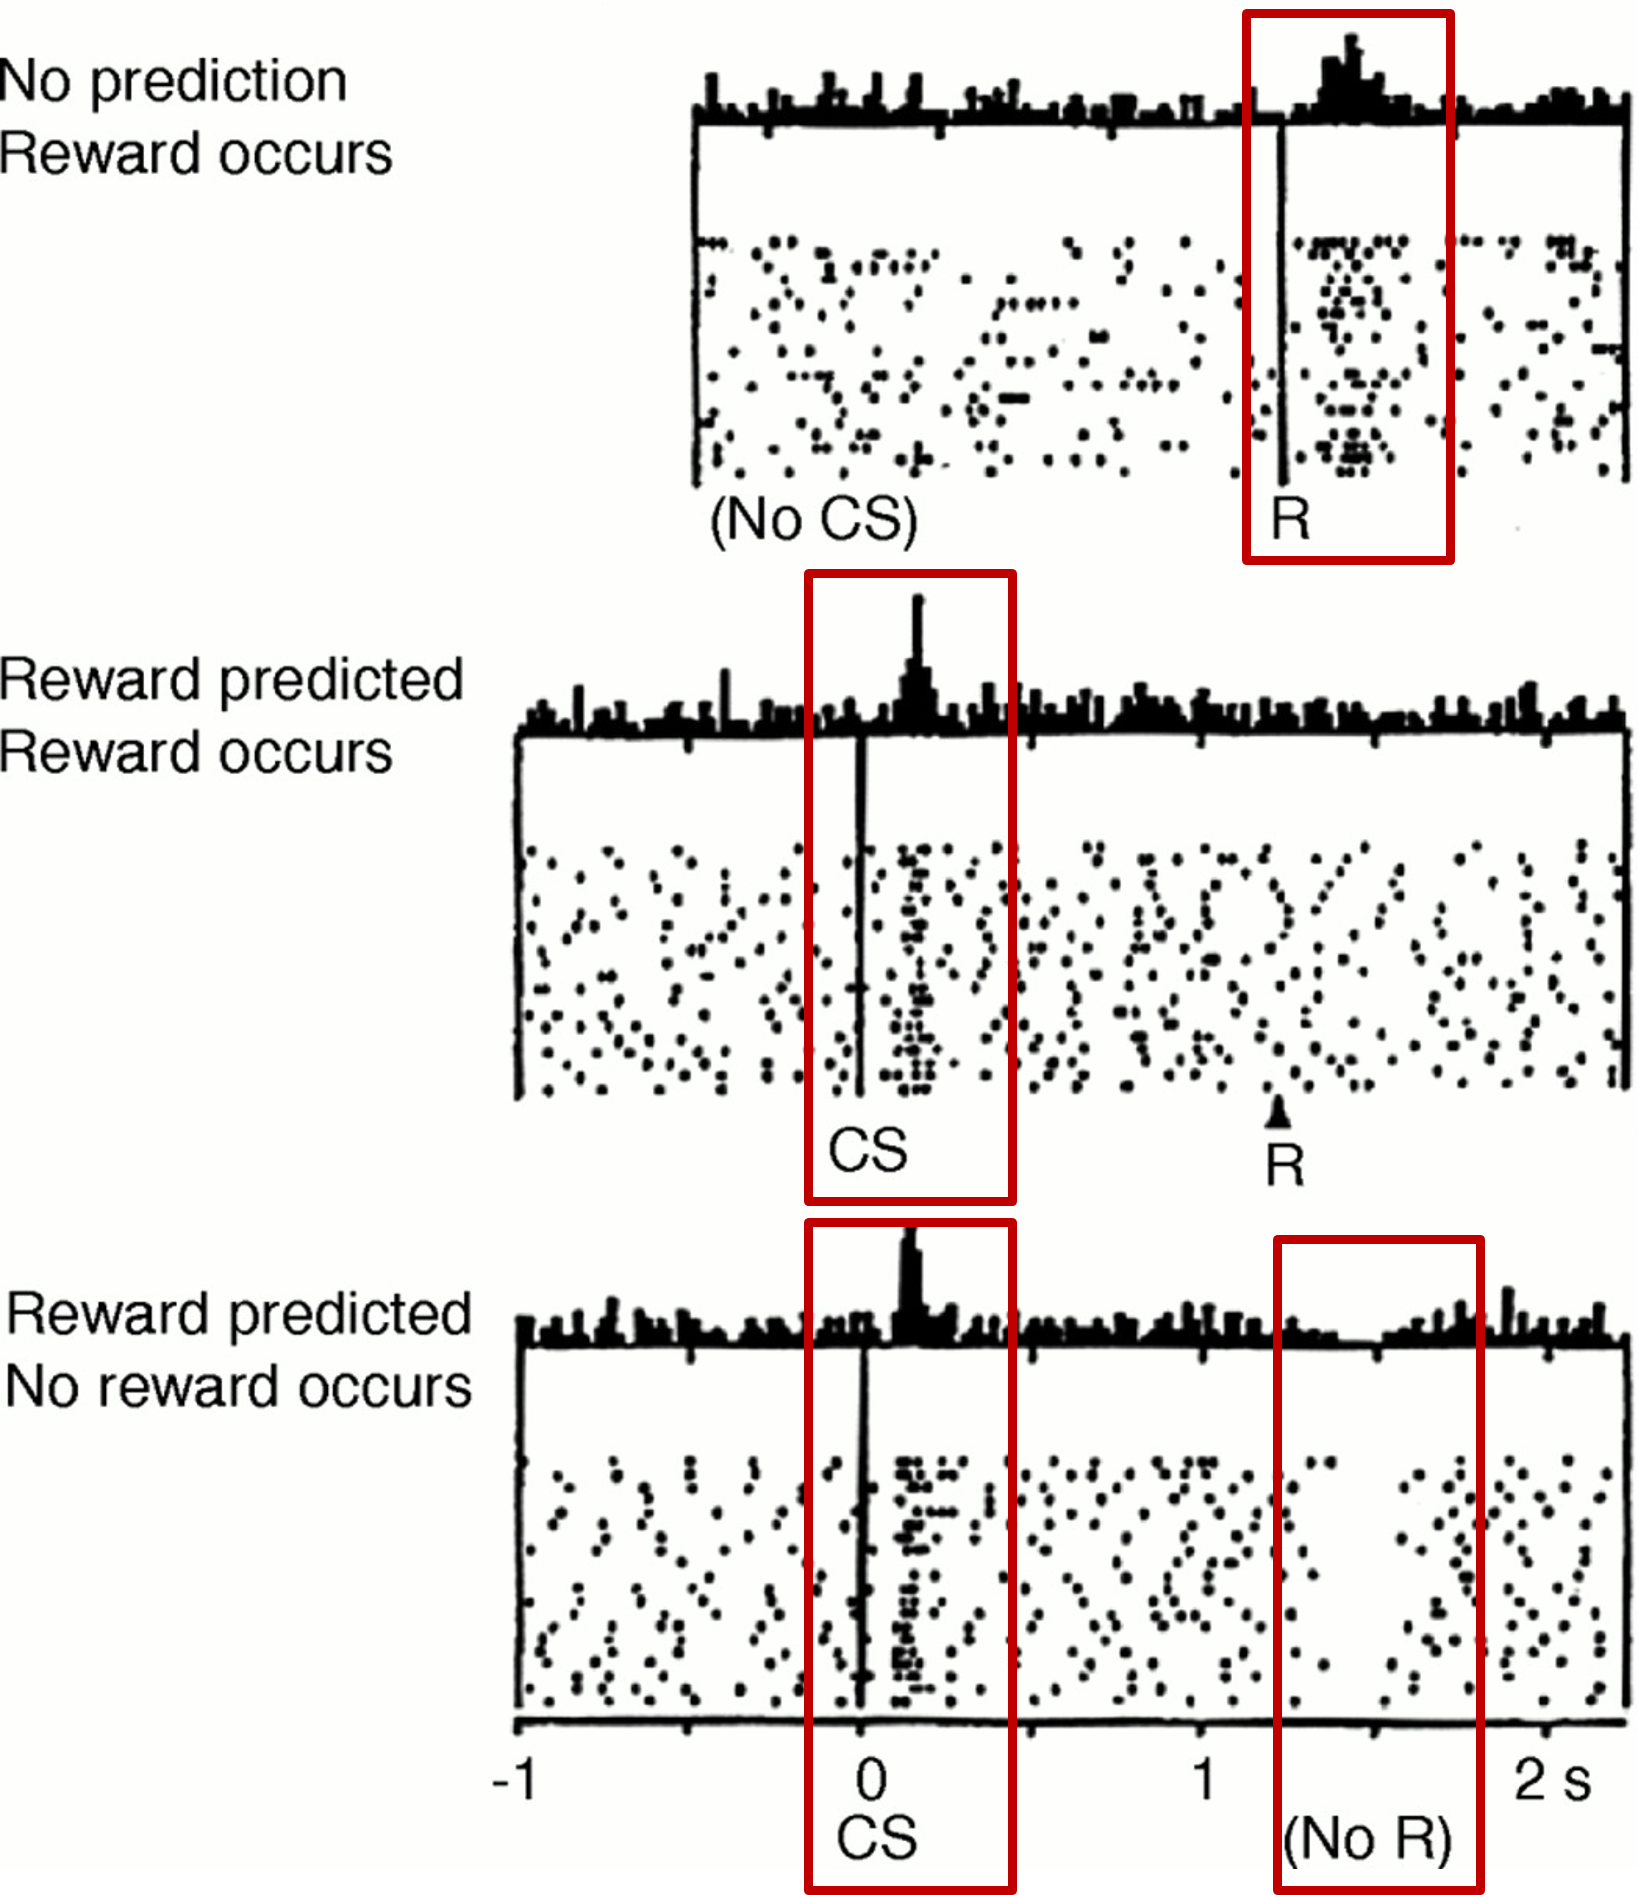
\includegraphics[width=0.8\linewidth]{../module1/img/dopamine_transfer_cs.png}
                        \end{subfigure}
                        \begin{subfigure}{0.48\linewidth}
                            \centering
                            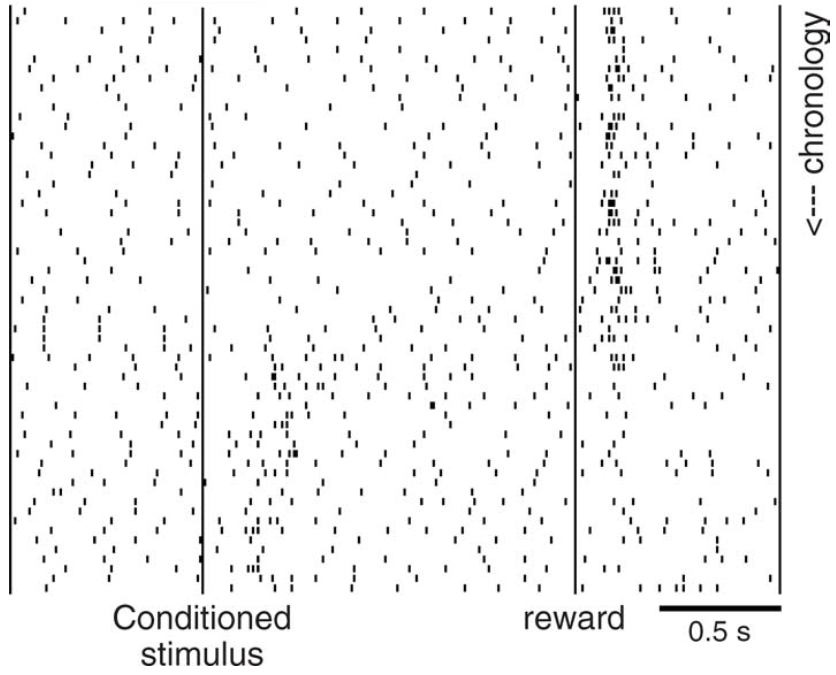
\includegraphics[width=0.9\linewidth]{./img/dopamine_transfer.png}
                        \end{subfigure}
                    \end{figure}
                \end{casestudy}


            \item[Probability encoding] \marginnote{Probability encoding}
                The dopaminergic response varies with the reward probability.

                \begin{casestudy}[Dopamine probability encoding \cite{dopamine_probability}]
                    It has been shown that dopamine responds differently based on the probability of receiving a reward.
                    
                    For high uncertainty (50\% probability of reward), a tonic response that starts from the CS and grows up to the reward time has been observed.

                    \begin{figure}[H]
                        \centering
                        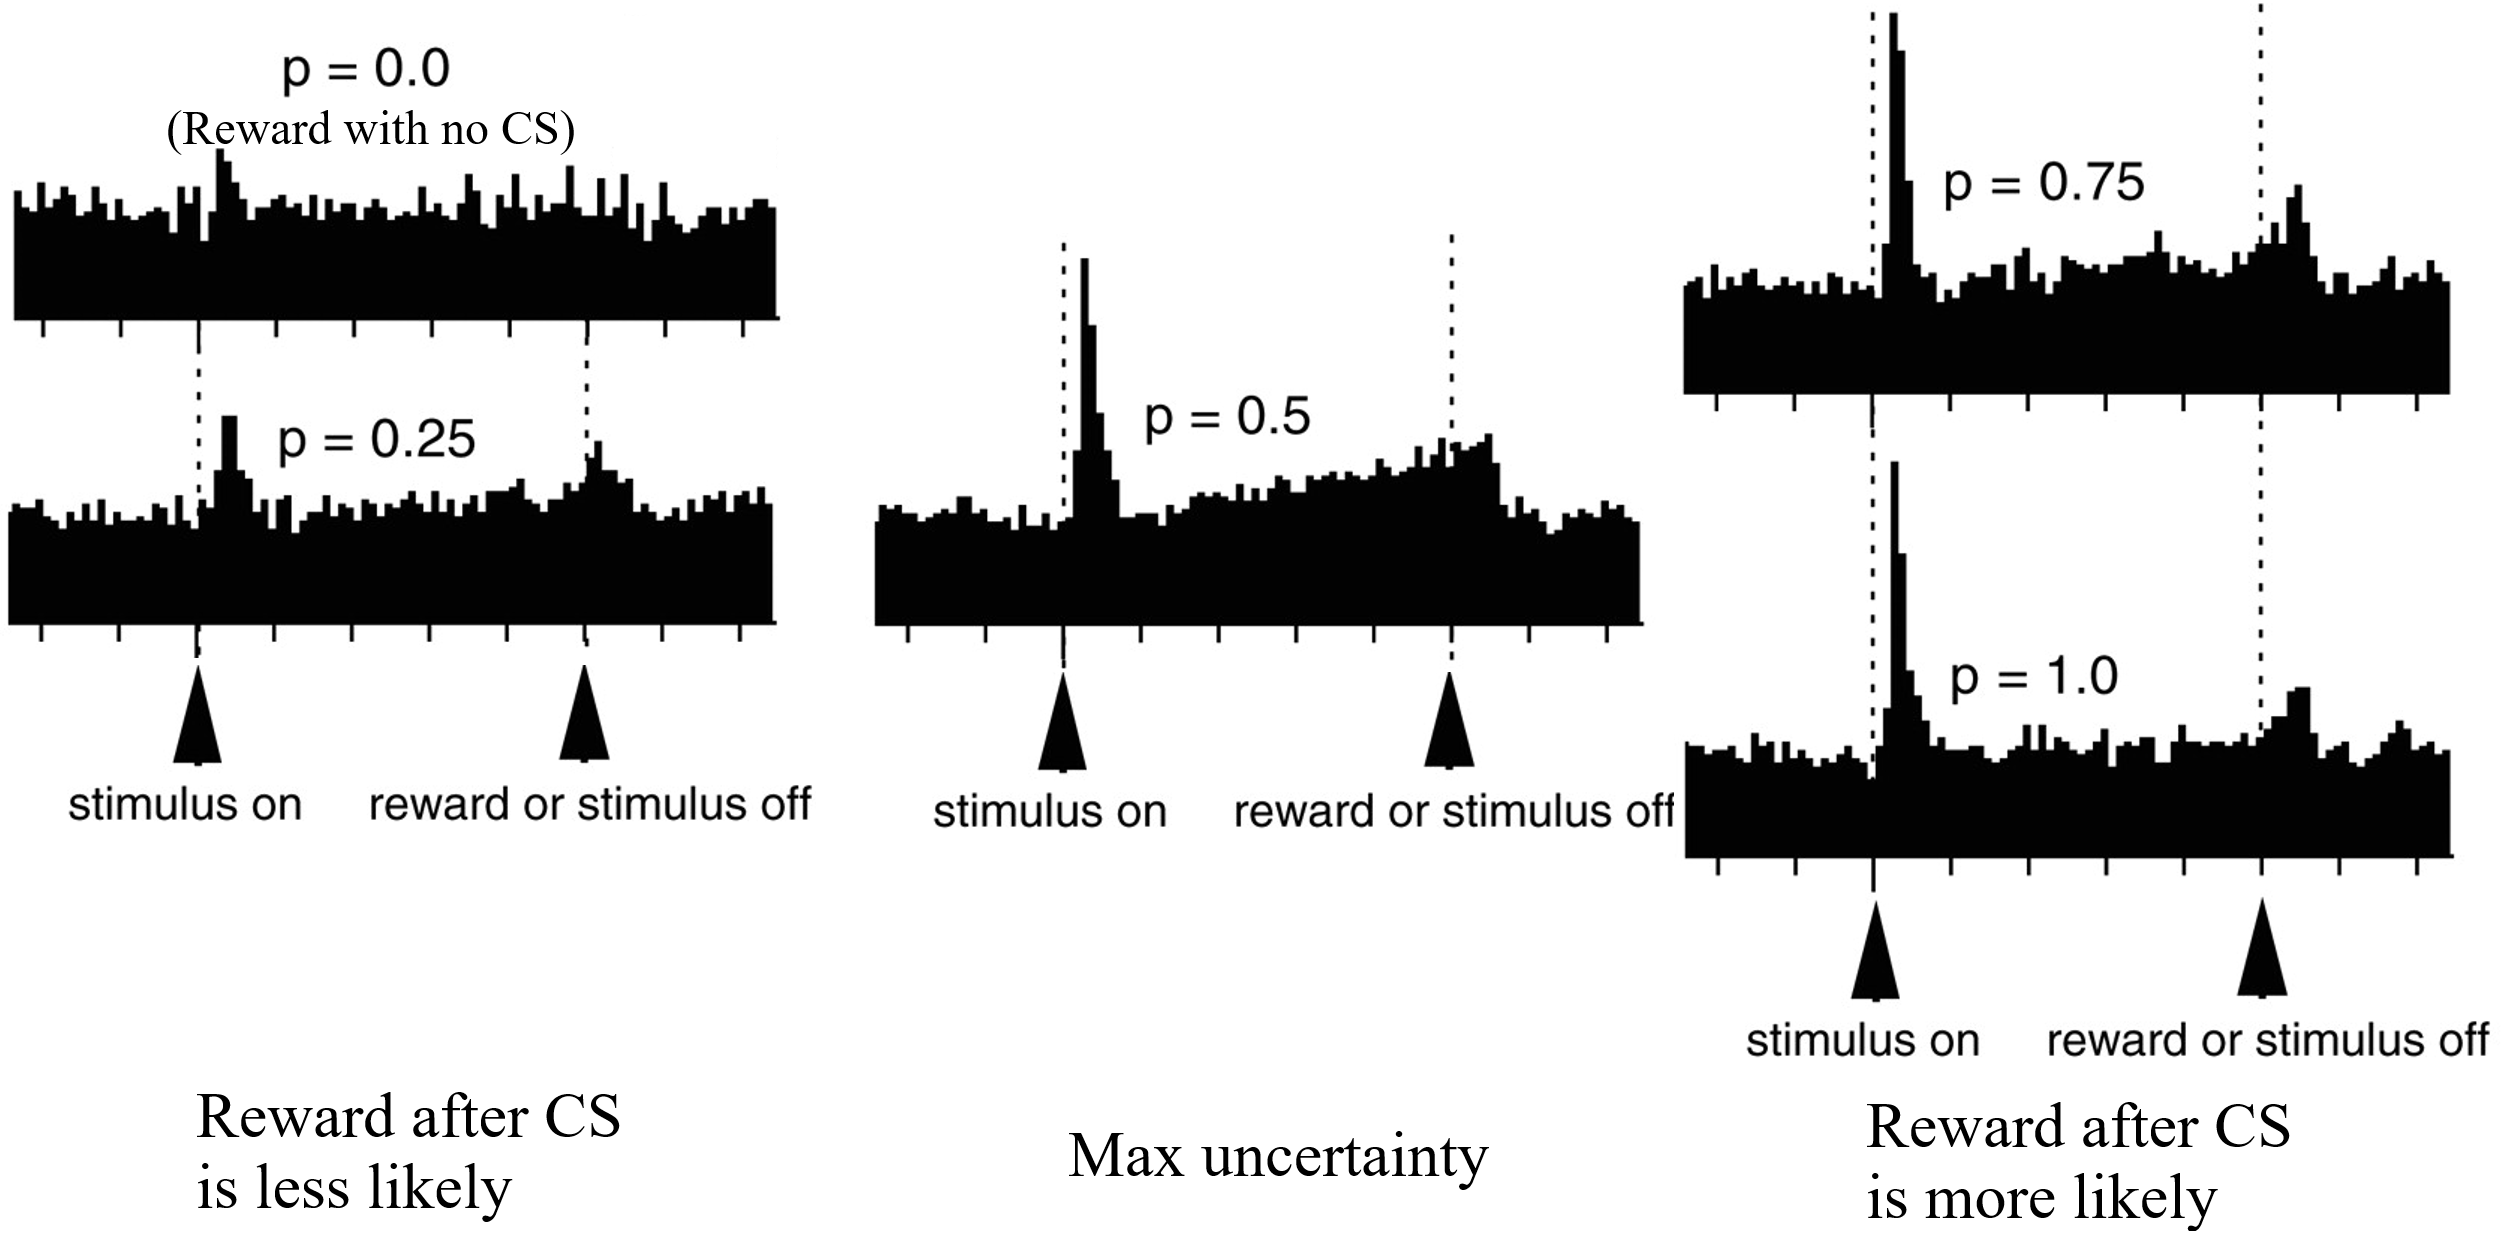
\includegraphics[width=0.8\linewidth]{../module1/img/dopamine_probability.png}
                    \end{figure}
                \end{casestudy}


            \item[Temporal prediction] \marginnote{Dopamine temporal prediction}
                Apart from encoding the unexpectedness of an event occurring, dopamine also accounts for the time the reward is expected to be delivered,
                and responds accordingly if the delivery happens earlier or later.

                \begin{casestudy}[Dopamine temporal prediction \cite{dopamine_temporal}]
                    It has been shown that dopamine responds differently based on the time the reward is delivered.

                    If the delivery happens earlier, the dopaminergic response increases.
                    On the other hand, if the delivery happens later, dopamine neurons first pass a depressed phase.

                    \begin{figure}[H]
                        \centering
                        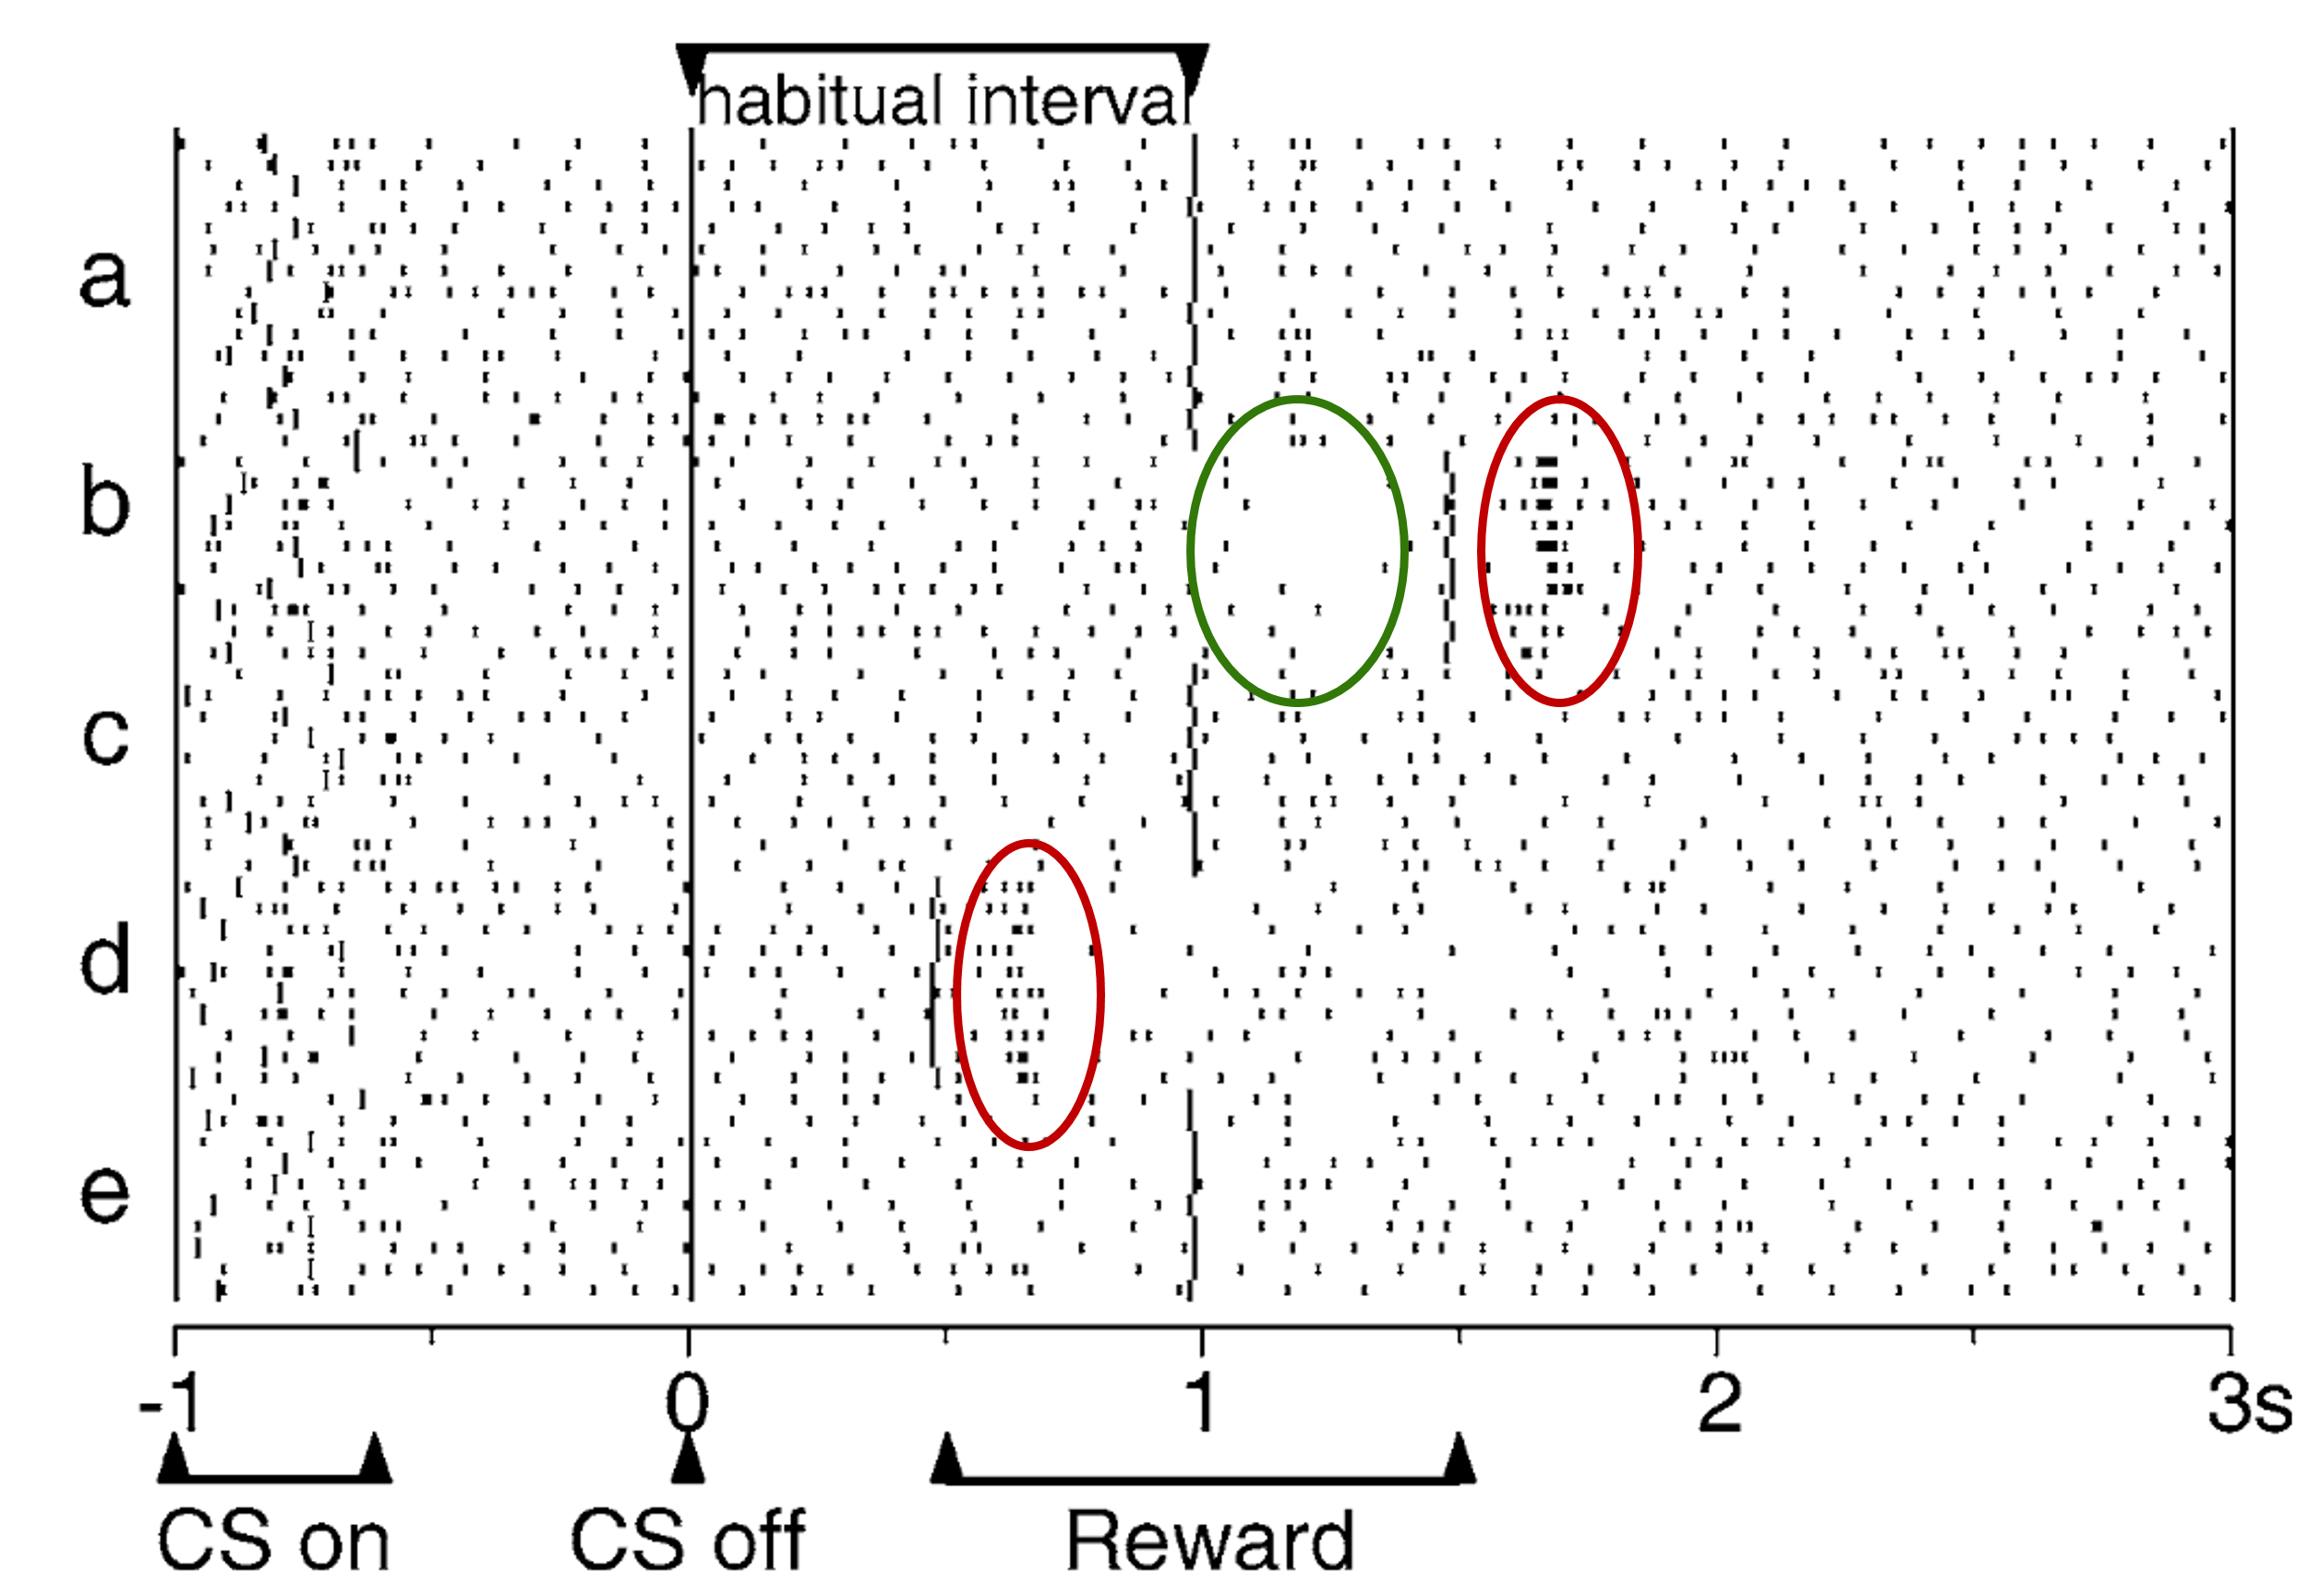
\includegraphics[width=0.45\linewidth]{../module1/img/dopamine_timing.png}
                    \end{figure}
                \end{casestudy}
    \end{description}
\end{description}

\begin{figure}[H]
    \centering
    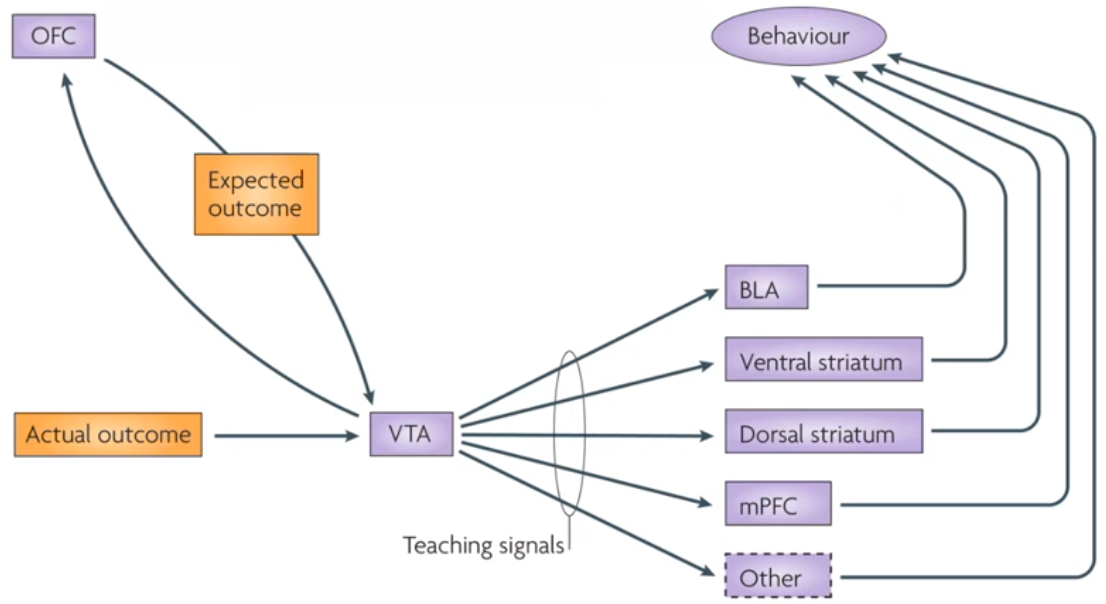
\includegraphics[width=0.7\linewidth]{./img/dopamine_flow.png}
    \caption{Dopamine flow in the dopaminergic system}
\end{figure}

\begin{remark}[PFC neurons]
    Differently from dopamine neurons, PFC neurons during learning fire in response to the reward and progressively start to fire also at the CS.
    In addition, the strength of the response does not depend on the expectedness of the reward 
    (i.e. it only acts as a prediction for the reward and not for the error).

    \begin{figure}[H]
        \centering
        \begin{subfigure}{0.34\linewidth}
            \centering
            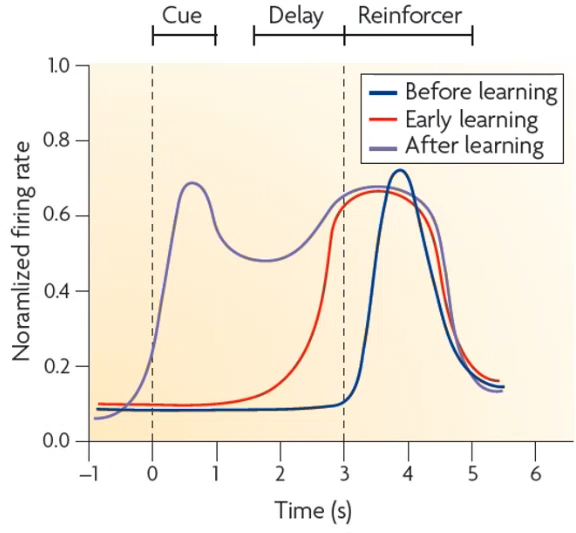
\includegraphics[width=0.9\linewidth]{./img/pfc_learning.png}
            \caption{PFC response during learning}
        \end{subfigure}
        \begin{subfigure}{0.62\linewidth}
            \centering
            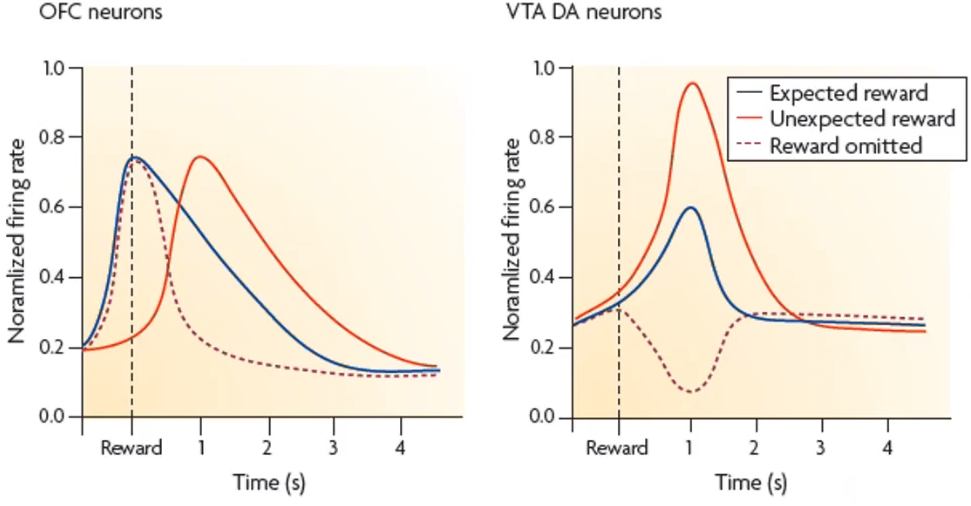
\includegraphics[width=0.9\linewidth]{./img/pfc_vs_dopamine.png}
            \caption{PFC vs dopamine (DA)}
        \end{subfigure}
    \end{figure}
\end{remark}



\section{Reward prediction error (RPE) theory of dopamine}


\subsection{Dopamine is not fully model-free}

There is strong evidence that midbrain dopamine is used to report RPE as in model-free RL.
RPE theory of dopamine states that:
\begin{itemize}
    \item Dopamine reflects the value of the observable state, which can be seen as a quantitative summary of future reward.
    \item State values are directly learned through experience.
    \item Dopamine only signals surprising events that bring a reward.
    \item Dopamine does not make inferences on the model of the environment.
\end{itemize}

However, individuals also learn about the model of the world (e.g. cognitive map) and this knowledge can affect the neuronal prediction error,
but, there is evidence that this acquisition involves cortical signals (e.g. PFC) rather than dopamine.
Despite that, dopamine still seems to integrate predictive information from models.

\begin{casestudy}[Monkey saccade \cite{saccade}]
    Monkeys are required to solve a memory-guided saccade task where, after fixation, 
    a light is flashed in one of the four directions indicating the saccade to be made after the fixation point went off.
    \begin{figure}[H]
        \centering
        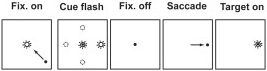
\includegraphics[width=0.4\linewidth]{./img/saccade1.png}
        \caption{Structure of the task}
    \end{figure}

    Experiments are done in sub-blocks of four trials, each corresponding to a direction.
    Moreover, the probability of reward increases with the number of non-rewarded trials (post-reward trial number, \texttt{PNR}).
    If $\texttt{PNR} = 1$, the probability of reward is the lowest ($0.0625)$, while if $\texttt{PNR} = 7$, the reward probability is $1.0$.
    \begin{figure}[H]
        \centering
        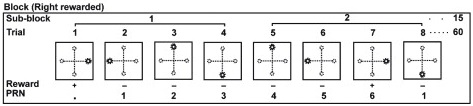
\includegraphics[width=0.6\linewidth]{./img/saccade2.png}
        \caption{Structure of a block}
    \end{figure}


    It is expected that the animal's reward prediction increases after each non-rewarded trial.
    In other words, as the reward is more likely after each non-rewarded trial, positive prediction error should decrease and 
    negative prediction error should be stronger (i.e. decrease).

    Results show that dopamine neurons are less active if the reward is delivered
    and more depressed if the reward is omitted after each non-rewarded trial.
    \begin{figure}[H]
        \centering
        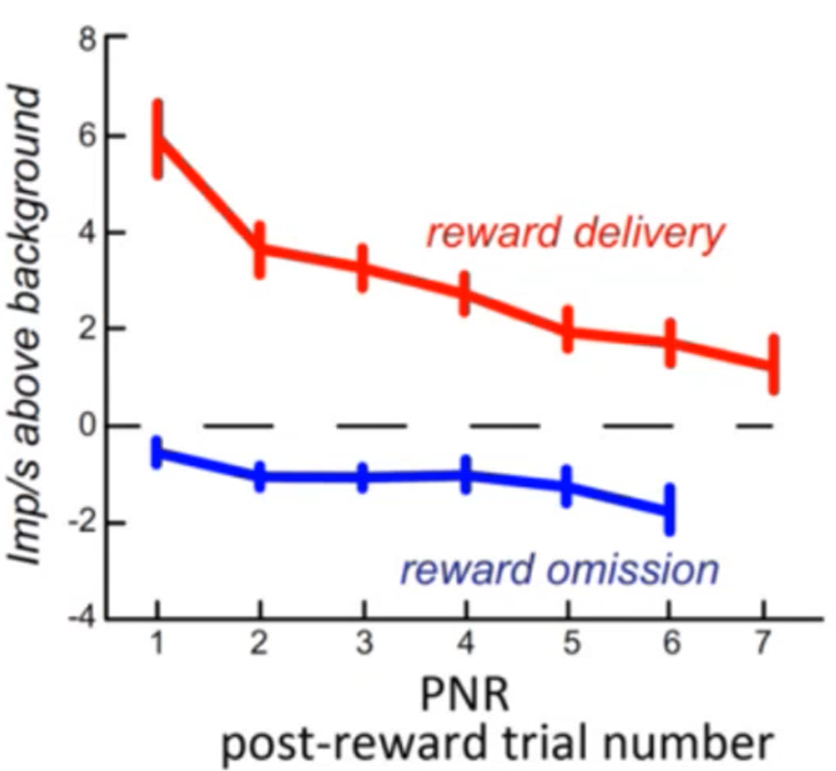
\includegraphics[width=0.25\linewidth]{./img/saccade3.png}
    \end{figure}

    The results are in contrast with an exclusive model-free view of dopamine as, if this were the case, 
    learning would only involve past non-rewarded trials causing positive prediction error to decrease and negative prediction error to be weaker (i.e. increase).
    Therefore, dopamine might process prediction error in both model-free and model-based approaches.
\end{casestudy}

\begin{casestudy}[Dopamine indirect learning \cite{indirect_learning}]
    Rats are exposed to:
    \begin{descriptionlist}
        \item[Pre-conditioning] Sound stimuli $A \mapsto B$ and $C \mapsto D$ are paired together.
        \item[Conditioning] The stimulus $B$ is paired with a reward. 
    \end{descriptionlist}
    Results show that rats respond to both $B$ and $A$ in a correlated manner.

    \begin{figure}[H]
        \centering
        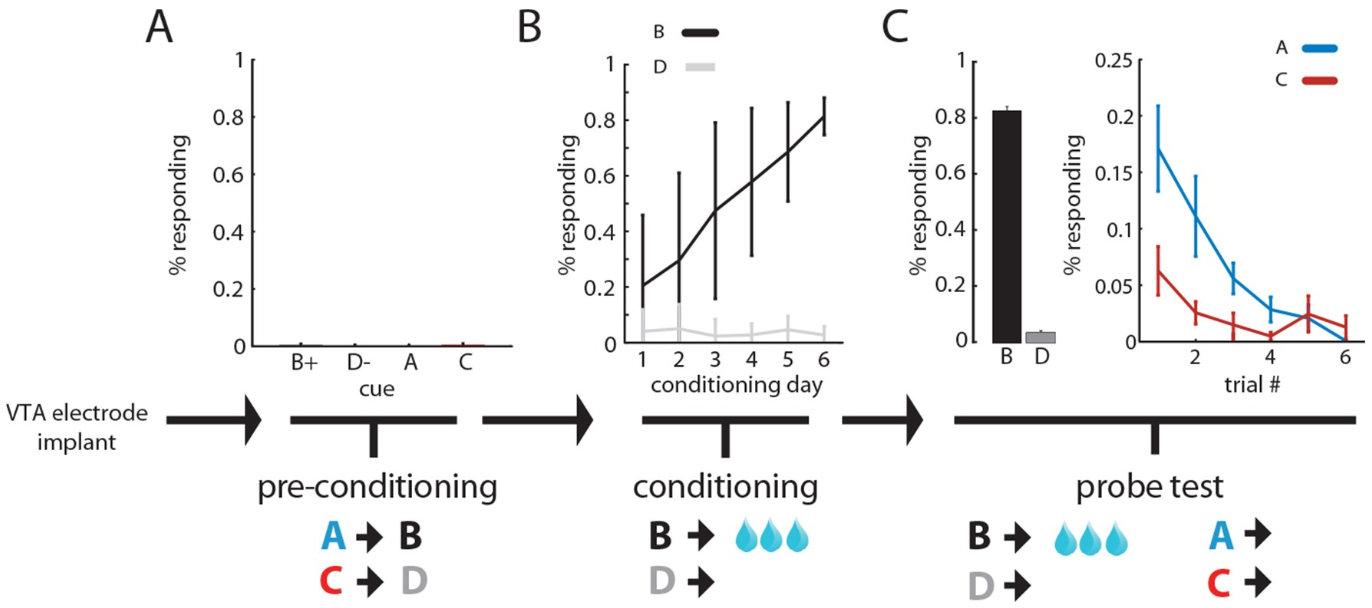
\includegraphics[width=0.65\linewidth]{./img/dopamine_indirect1.png}
    \end{figure}

    \begin{figure}[H]
        \centering
        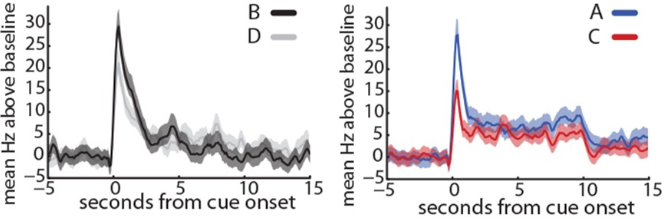
\includegraphics[width=0.45\linewidth]{./img/dopamine_indirect2.png}
    \end{figure}

    The results show that dopamine might also reflect values learned indirectly.
    This is in contrast with the temporal difference learning of model-free RL in which only directly experienced states are learned.
\end{casestudy}

\begin{casestudy}[Dopamine RPE reflects inference over hidden states \cite{dopamine_hidden}]
    Rats are trained to associate odors with rewards.
    Two types of tasks are considered:
    \begin{descriptionlist}
        \item[Task 1] 
            Odors are always associated with a reward. 
            Odor $A$ is delivered with a delay sampled from a Gaussian distribution, odors $B$ and $C$ are deterministic and odor $D$ is for control.

        \item[Task 2] 
            As above, but odors are associated with a reward $90\%$ of the time. 
    \end{descriptionlist}
    The period in which no reward is expected is called ITI, while the period in which the animal expects a reward is the ISI (i.e. after the odor onset).

    \begin{figure}[H]
        \centering
        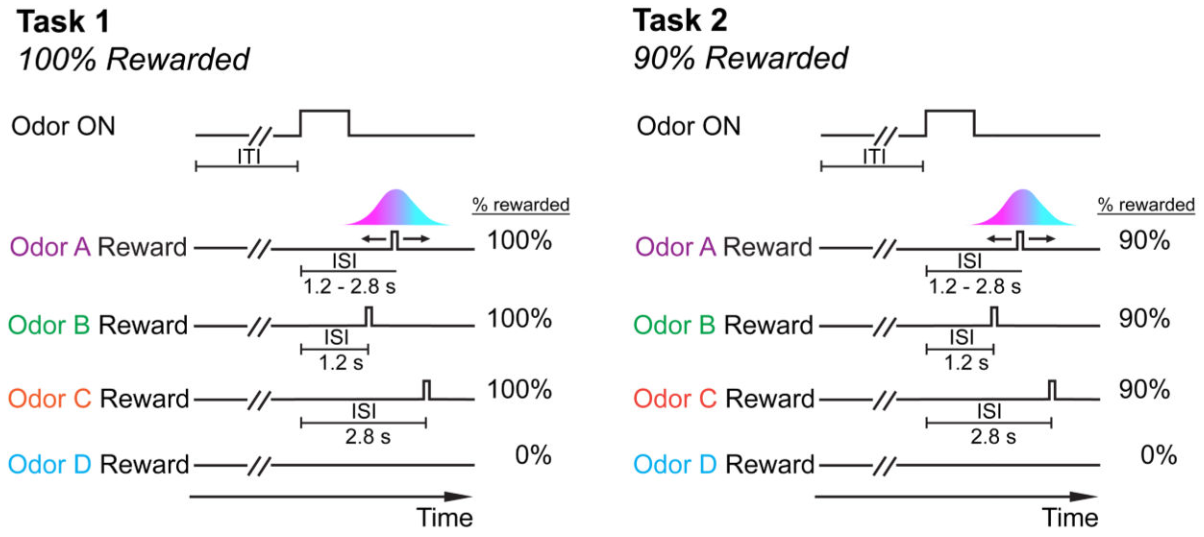
\includegraphics[width=0.65\linewidth]{./img/dopamine_hidden1.png}
        \caption{Tasks representation}
    \end{figure}

    \begin{figure}[H]
        \centering
        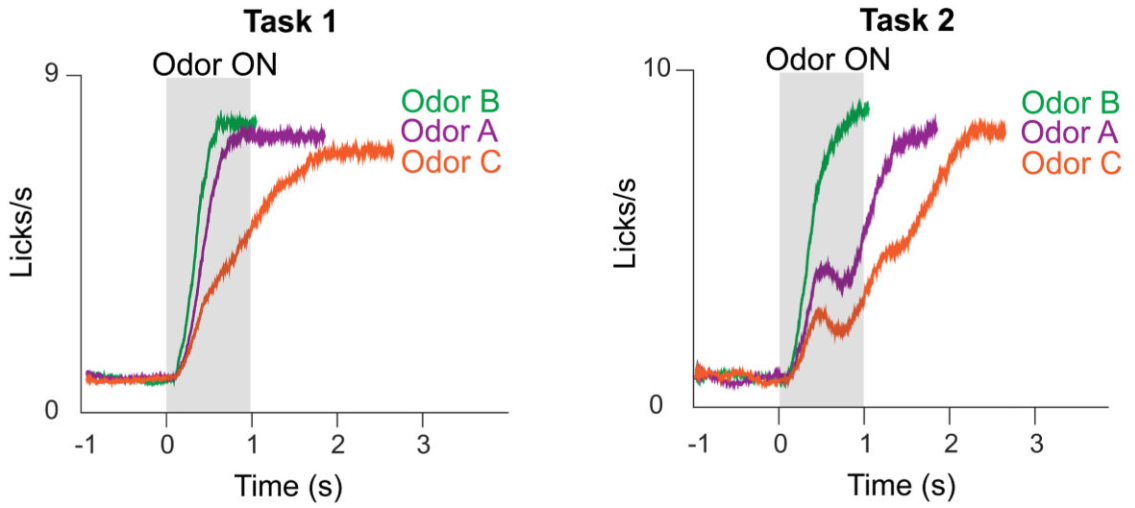
\includegraphics[width=0.5\linewidth]{./img/dopamine_hidden2.png}
        \caption{
            \parbox[t]{0.7\linewidth}{
                Licking behavior in the two tasks.
                It can be seen that, for each odor, licking depends on the time of arrival of the reward.
                On task 2, licking is more uncertain.
            }
        }
    \end{figure}

    Considering odor $A$, results show that:
    \begin{itemize}
        \item For task 1, the dopaminergic response gets smaller over time within the ISI
        \item For task 2, the dopaminergic response grows, hinting at the fact that some sort of inference about the state is being made.
    \end{itemize} 
    \begin{figure}[H]
        \centering
        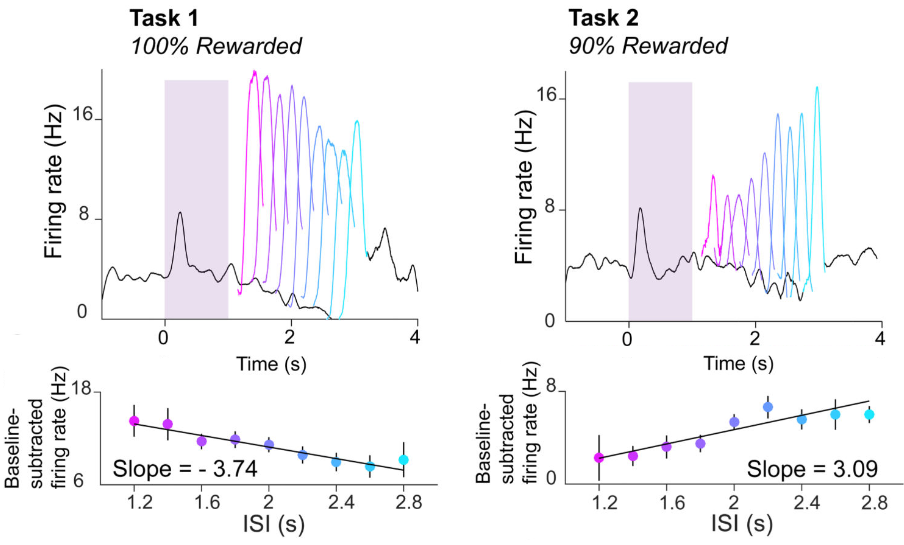
\includegraphics[width=0.65\linewidth]{./img/dopamine_hidden3.png}
    \end{figure}

    An explanation is that the animal has to solve the problem of determining whether it is in an ITI or ISI period:
    \begin{itemize}
        \item For task 1, the rat can easily determine in which period it is.
        \item For task 2, as the reward is not always delivered, being in ISI and ITI is not always clear.
    \end{itemize}
    \begin{figure}[H]
        \centering
        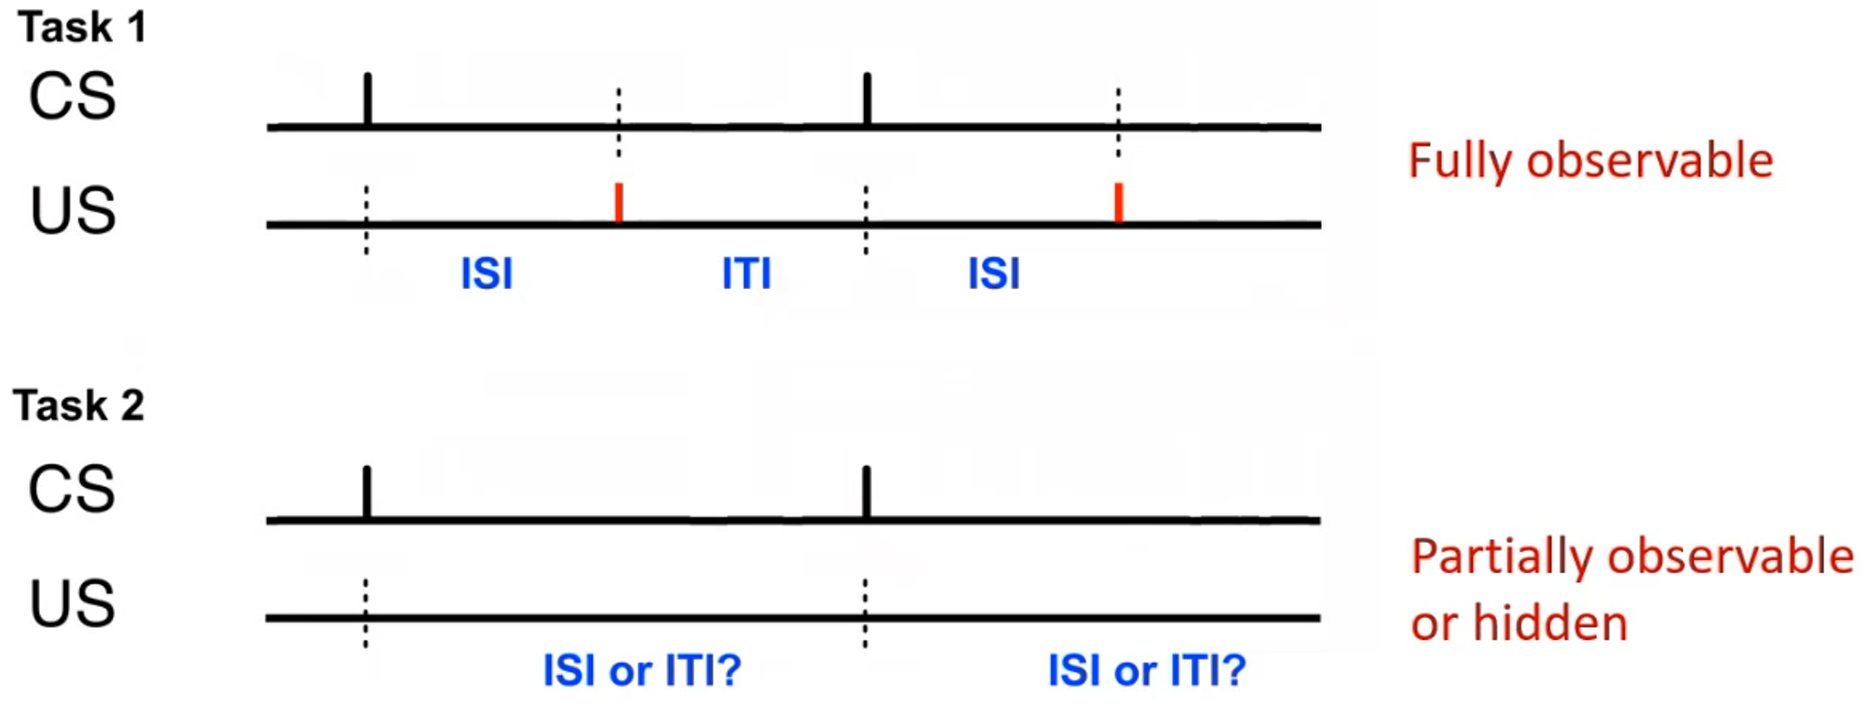
\includegraphics[width=0.5\linewidth]{./img/dopamine_hidden4.png}
    \end{figure}

    The dopaminergic activity for the two tasks can be explained as follows:
    \begin{itemize}
        \item For task 1, after the stimulus, the probability of receiving a reward increases over time.
            Therefore, the RPE is increasingly suppressed.
        \item For task 2, as the reward fails to arrive, the belief state progressively shifts towards the ITI state.
            Therefore, if the reward is delivered later, the RPE is high as it was unexpected.
    \end{itemize}
    \begin{figure}[H]
        \centering
        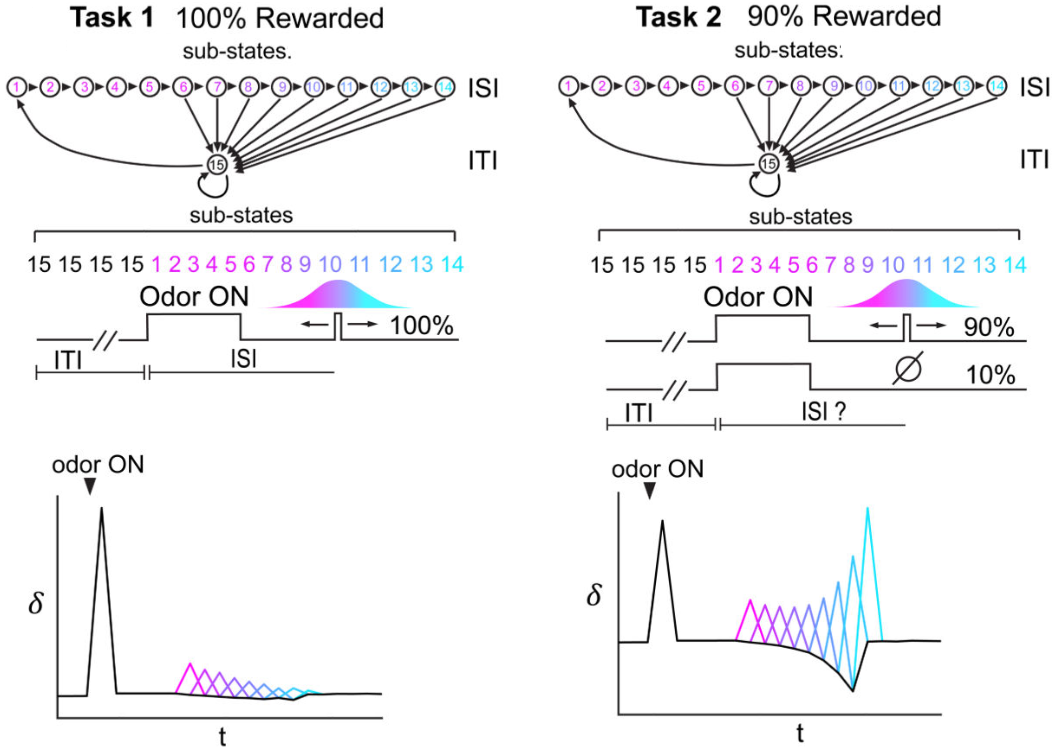
\includegraphics[width=0.55\linewidth]{./img/dopamine_hidden5.png}
        \caption{
            \parbox[t]{0.6\linewidth}{
                Experiment represented as sub-states (top) and RPE to a reward over time (bottom)
            }
        }
    \end{figure}

    These results hint at the fact that:
    \begin{itemize}
        \item The brain is not limited to passively observing the environment but also makes latent inferences.
        \item The results can be modeled using a temporal difference model that incorporates hidden-state inference.
    \end{itemize}
\end{casestudy}


\subsection{Dopamine as generalized prediction error}

Dopamine might not be limited to only predicting reward error but is also involved in a more general state prediction error.

\begin{casestudy}[Dopamine state change prediction \cite{dopamine_general}]
    Rats are exposed to the following training steps:
    \begin{descriptionlist}
        \item[Conditioning] 
            The following stimuli are associated with some rewards
            (it must be ensured that rewards are liked in the same way, i.e. same value but different identity):
            \begin{itemize}
                \item $V_B$ is associated with two units of banana.
                \item $V_{UB}$ is associated with two units of chocolate.
            \end{itemize}

        \item[Compound training]
            New stimuli are paired with the previously learned ones:
            \begin{itemize}
                \item $A_B$ is paired with $V_B$. Because of blocking, $A_B$ should not be learned as a rewarding stimulus.
                \item $A_{UB}$ is paired with $V_{UB}$. The reward is changed to achieve identity unblocking.
            \end{itemize}
    \end{descriptionlist}

    \begin{figure}[H]
        \centering
        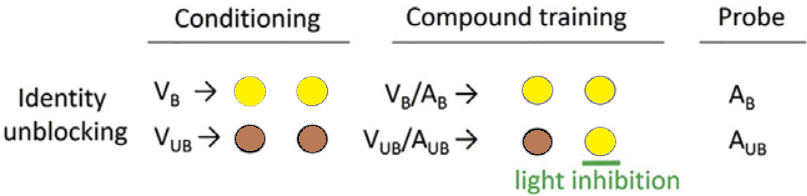
\includegraphics[width=0.6\linewidth]{./img/dopamine_general1.png}
    \end{figure}

    It has been shown that the animal learns the new CS $A_{UB}$ and dopamine responds to the change even if only the identity of the reward changed and the value remained the same.
\end{casestudy}


\subsection{Successor representation}

\begin{description}
    \item[Sensory prediction error (SPE)] \marginnote{Sensory prediction error (SPE)}
        Generalized prediction error over sensory features that estimates the successor representation of a state.

    \item[Successor representation (SR)] \marginnote{Successor representation (SR)}
        The SR of a state $s$ is a mapping $M(s, \cdot)$ where $M(s, s')$ indicates the expected occupancy of $s'$ by starting from $s$ 
        (i.e. how likely it is to end up in $s'$ from $s$).

        A SR learner predicts the value of a state by taking into account the reward $R$ and the successor representation $M$:
        \[ 
            V(s_t) = R(s_{t}) M(s_t, s_{t+1}) 
            \hspace{2em}
            \left( \text{\cite{sr_learner} says } V(s_t) = \sum_{t+1} R(s_{t+1}) M(s_t, s_{t+1}) \right)
        \]
        % A SR learner predicts the value of a state as \cite{sr_learner}:
        % \[ V(s_t) = \sum_{t+1} R(s_{t+1}) M(s_t, s_{t+1}) \]
\end{description}

\begin{remark}
    SR learning might be a middle ground between model-free and model-based methods.
    SR computes the future reward by combining the efficiency of model-free approaches and some flexibility from model-based RL (i.e. caching of state transitions).

    This is suited for tasks where the states are more or less stable but rewards and goals change frequently.
\end{remark}

\begin{remark}
    A criticism against this method is that it is space-wise expensive as it involves a prediction error for states (the matrix $M$).
    This space requirement finds a mismatch in the number of neurons available in the brain as 
    dopaminergic neurons, which are responsible for updating the values, might not be enough.
    \begin{figure}[H]
        \centering
        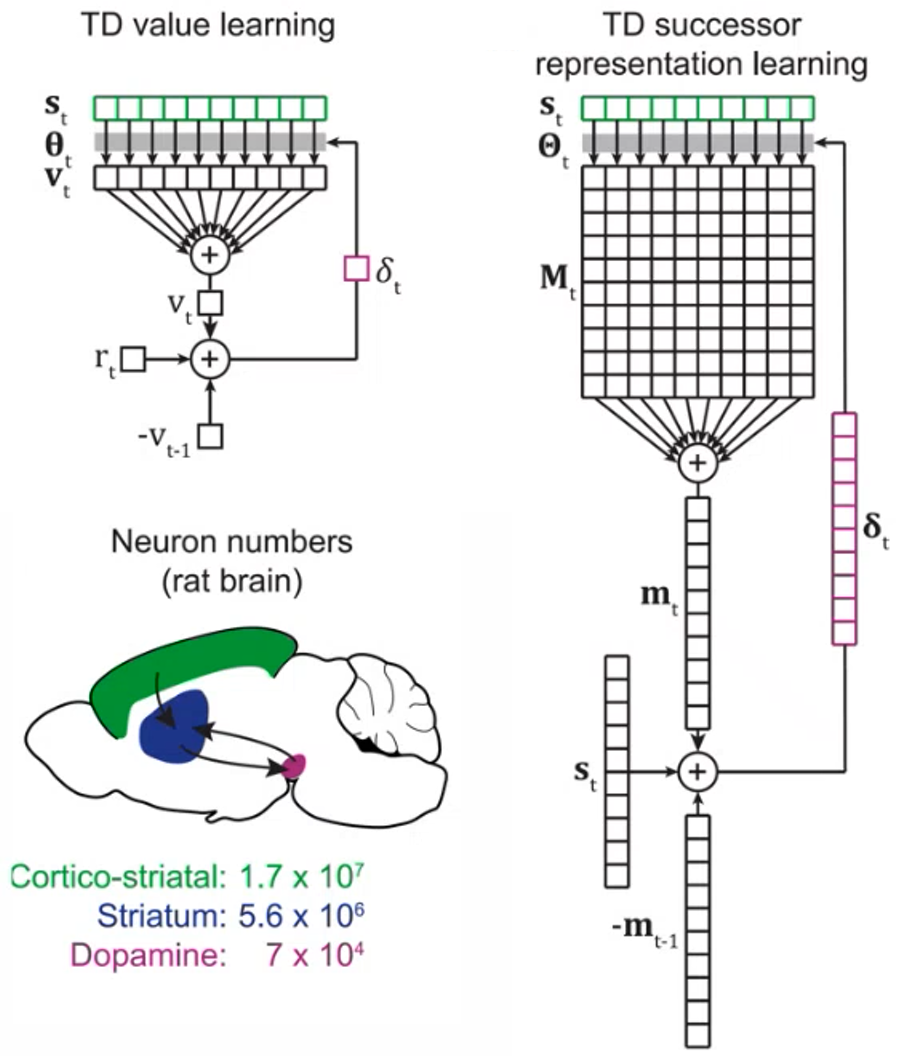
\includegraphics[width=0.4\linewidth]{./img/sr_mismatch.png}
    \end{figure}
\end{remark}

\begin{casestudy}[SR in humans \cite{sr_learner}]
    The experiment is divided into the following phases:
    \begin{descriptionlist}
        \item[Learning phase] 
            Candidates are exposed to a sequence of three stimuli, where the third is associated with a reward.
            After a bunch of trials (with different stimuli), they are asked to indicate which starting stimulus is the one leading to the greater future reward.

        \item[Re-learning phase]
            Two types of revaluation are considered:
            \begin{descriptionlist}
                \item[Reward revaluation] 
                    Final rewards are swapped with the stimuli unchanged (i.e. value change).
                \item[Transition revaluation] 
                    Third stimuli are swapped with the rewards unchanged (i.e. state change). 
            \end{descriptionlist}
            Candidates are again exposed to the sequence of stimuli starting from the middle one (i.e. the first stimulus is dropped).
            
            Expected results are:
            \begin{itemize}
                \item Model-free approaches should fail on both changes.
                \item Model-based approaches should succeed in both changes.
                \item SR-based approaches should succeed in the reward change but not in the transition change.
            \end{itemize}
    \end{descriptionlist}

    \begin{figure}[H]
        \centering
        \begin{subfigure}{0.48\linewidth}
            \centering
            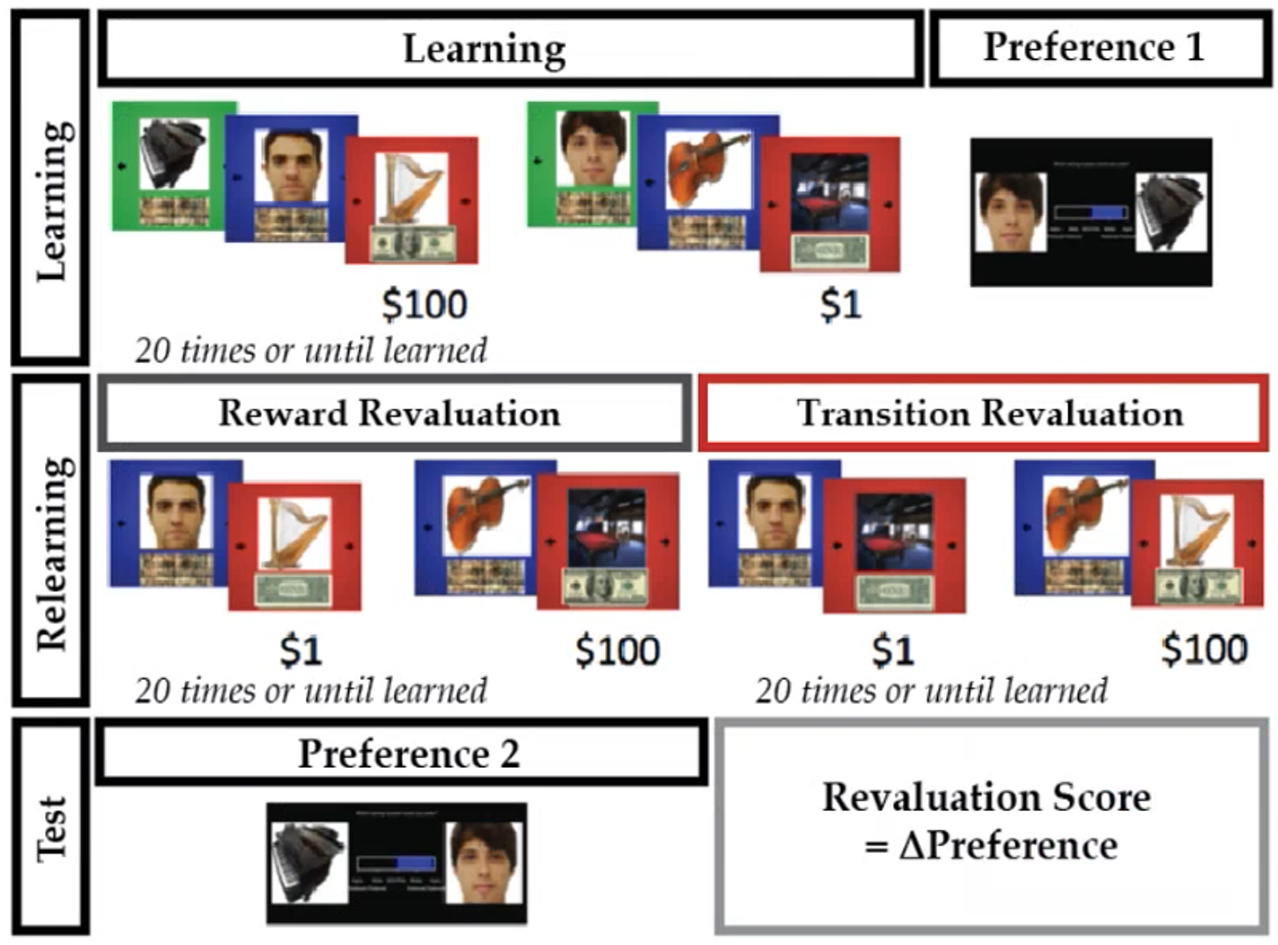
\includegraphics[width=0.9\linewidth]{./img/human_sr1.png}
        \end{subfigure}
        \begin{subfigure}{0.48\linewidth}
            \centering
            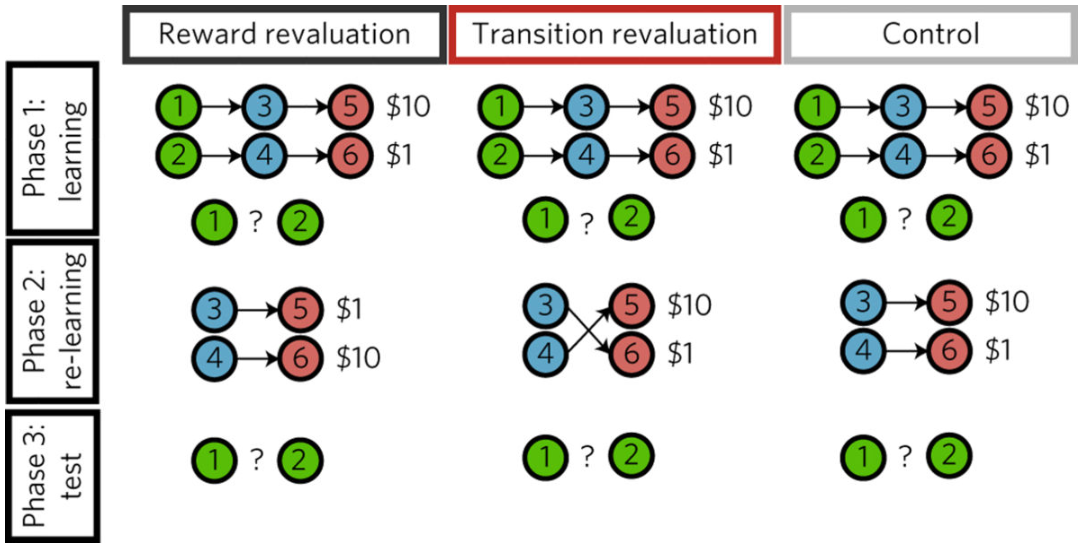
\includegraphics[width=0.95\linewidth]{./img/human_sr2.png}
        \end{subfigure}
    \end{figure}

    Results show that:
    \begin{itemize}
        \item Revaluation scores (i.e. change in preference) on reward revaluation are slightly better than transition revaluation.
        \item Reaction time for reward revaluation is faster (cached rewards can be easily updated) but 
            slower for the transition revaluation (cannot rely on cached states as they require more time to be updated).
    \end{itemize} 
    This suggests that humans might use successor representation learning with some form of model-based approach.
    Because of the differences in score and reaction time, learning cannot be fully model-based.

    \begin{figure}[H]
        \centering
        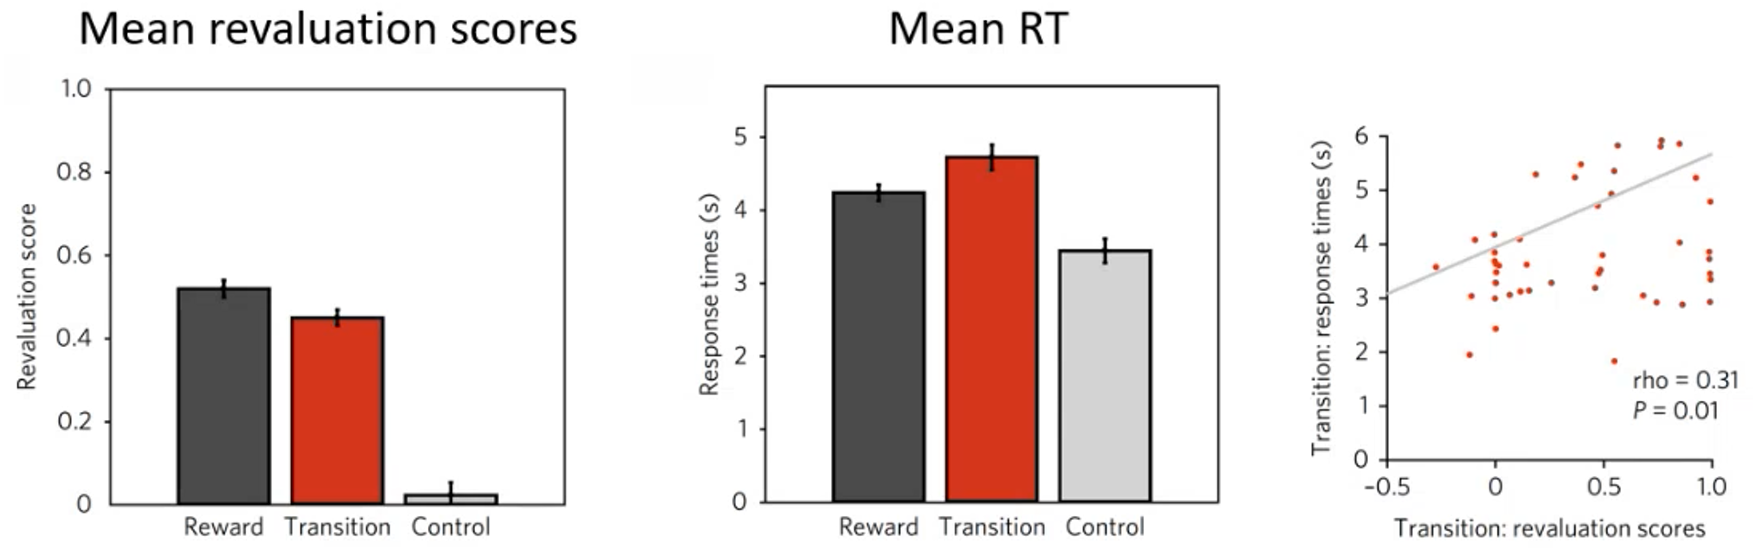
\includegraphics[width=0.6\linewidth]{./img/human_sr3.png}
    \end{figure}
\end{casestudy}



\section{Distributional reinforcement learning}

\begin{description}
    \item[Distributional reinforcement learning] \marginnote{Distributional reinforcement learning}
        RL methods that aim to learn the full distribution of the expected reward instead of the mean expected reward.
\end{description}

\begin{remark}
    Certain deep RL algorithms improve with distributional RL.
\end{remark}

\begin{remark}
    In traditional temporal-difference learning, predictors learn similar values.

    In distributional temporal-difference learning, there are optimistic and pessimistic predictors with different scaling
    that expect larger and smaller future rewards, respectively.

    \begin{figure}[H]
        \centering
        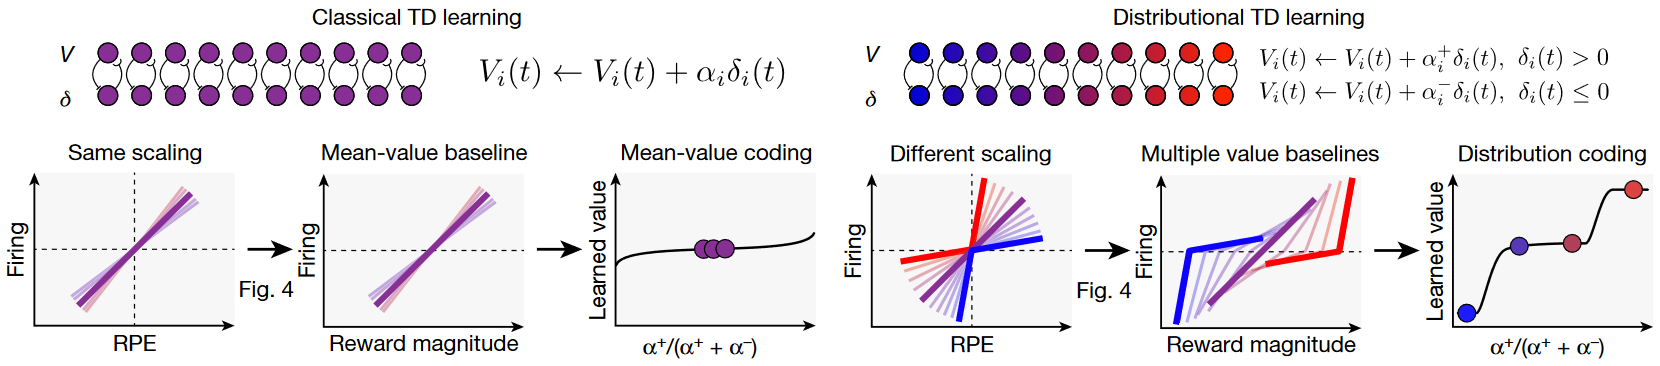
\includegraphics[width=0.9\linewidth]{./img/distr_rl1.png}
        \caption{
            \parbox[t]{0.9\linewidth}{
                Traditional RL (left) and distributional RL (right). In distributional RL, red nodes are optimistic and blue nodes are pessimistic.
            }
        }
    \end{figure}
\end{remark}

\begin{description}
    \item[Reversal point] \marginnote{Reversal point}
        $r_0$ is the reversal point of a dopaminergic neuron if:
        \begin{itemize}
            \item A reward $r < r_0$ expresses a negative error.
            \item A reward $r > r_0$ expresses a positive error.
        \end{itemize}

        \begin{remark}
            In traditional temporal-difference learning, the reversal point of individual neurons should be approximately identical.
        \end{remark}
\end{description}

\begin{casestudy}[Distributional RL in dopamine response \cite{distributional_rl_brain}]
    Single dopaminergic neurons are recorded in rats.
    Rats are trained on two different tasks:
    \begin{descriptionlist}
        \item[Variable-magnitude]
            A random amount of reward is given to the rat. The reward is anticipated by an odor stimulus in half of the trials.

        \item[Variable-probability]
            Three odor stimuli are each associated with a probability of reward (90\%, 50\%, 10\%).
            A control odor is associated with no reward.
    \end{descriptionlist}
    \begin{figure}[H]
        \centering
        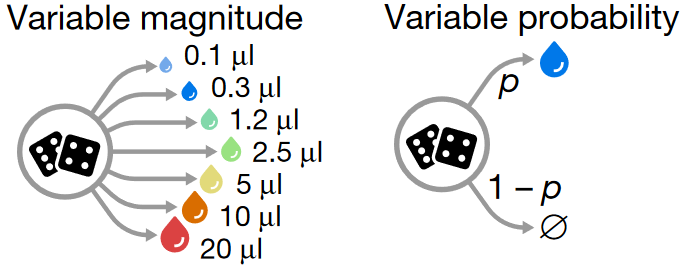
\includegraphics[width=0.4\linewidth]{./img/distr_rl2.png}
    \end{figure}

    Results on the variable-magnitude task show that:
    \begin{itemize}
        \item Neurons in simulated classical RL carry approximately the same RPE signal for each magnitude and have similar reversal points ($\sim 0$).
        \item Neurons in simulated distributional RL have different reversal points and there is more variety in responses 
            (e.g. RPEs of optimistic neurons are positive only for large magnitudes and vice versa for pessimistic neurons).
        \item Measured neural data are more similar to the simulated distributional RL data.
    \end{itemize}
    \begin{figure}[H]
        \centering
        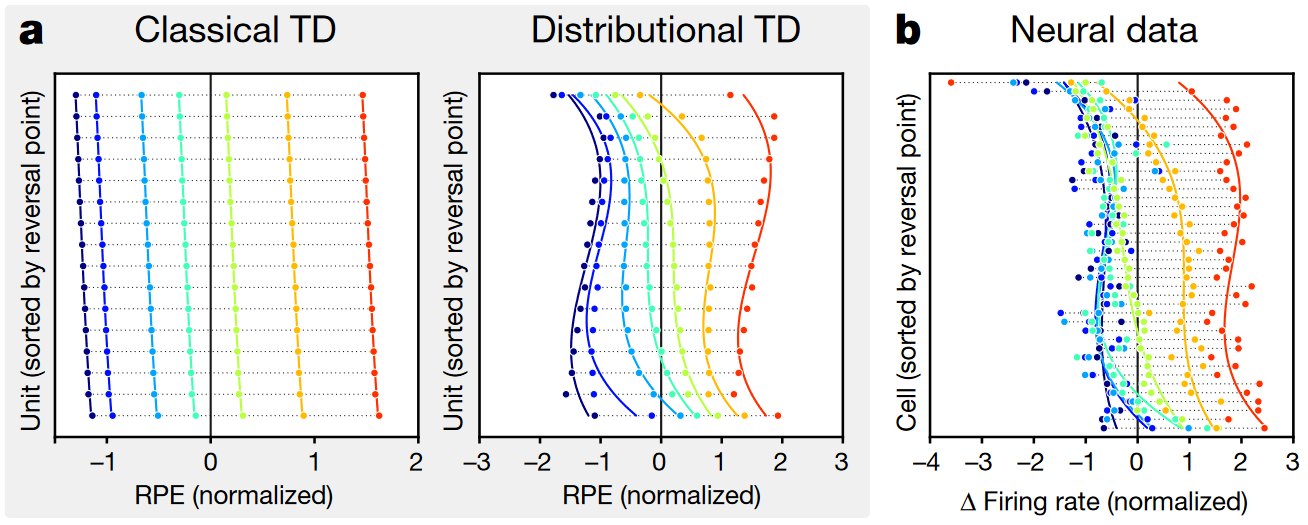
\includegraphics[width=0.7\linewidth]{./img/distr_rl3.png}
        \caption{
            \parbox[t]{0.7\linewidth}{
                Simulated (a) and measured (b) neurons.
                Points at the same y-axis represent the same neuron and are sorted by reversal point.
                The color of the dots represents the magnitude of the reward.
            }
        }
    \end{figure}

    Results on the variable-probability task show that:
    \begin{itemize}
        \item Neurons in simulated classical RL do not show differences when comparing the stimulus with 50\% reward against the 10\% and 90\% responses.
        \item Neurons in simulated distributional RL vary a lot when responding to the 50\% reward probability stimulus.
        \item Measured neural data are more similar to the simulated distributional RL data.
    \end{itemize}
    \begin{figure}[H]
        \centering
        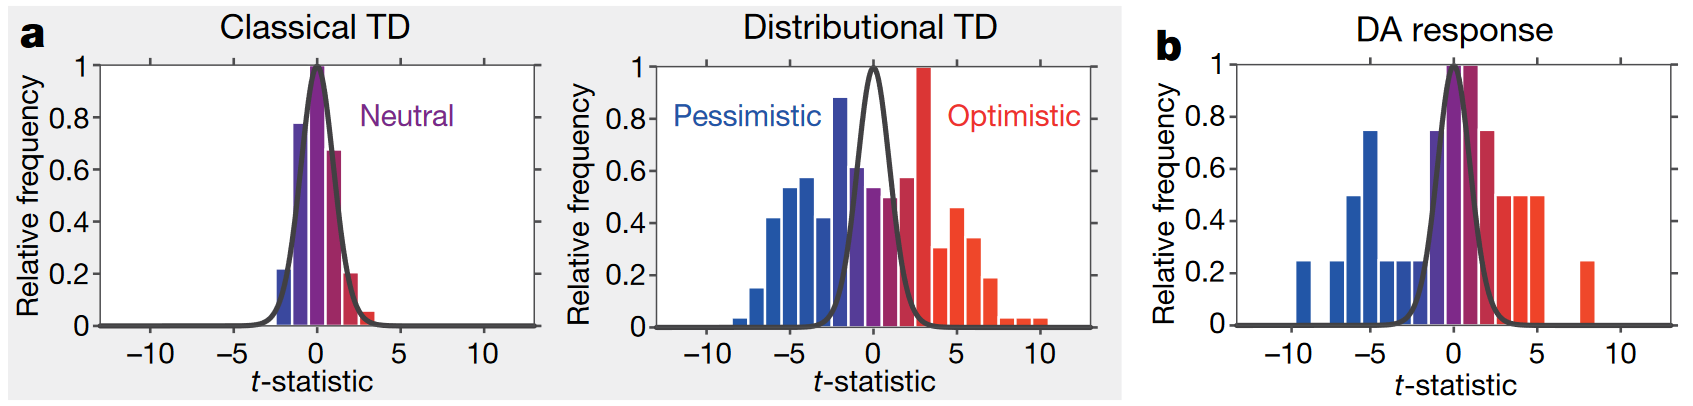
\includegraphics[width=0.7\linewidth]{./img/distr_rl4.png}
        \caption{
            \parbox[t]{0.7\linewidth}{
                Simulated (a) and measured (b) neurons.
                T-statistics comparing each cell's response to the stimulus associated with the 50\% reward
                against the mean stimulus response across cells.
            }
        }
    \end{figure}

    Responses of dopamine neurons show that some cells are in fact more optimistic and some more pessimistic
    depending on how they respond to the 50\% stimulus.
    \begin{figure}[H]
        \centering
        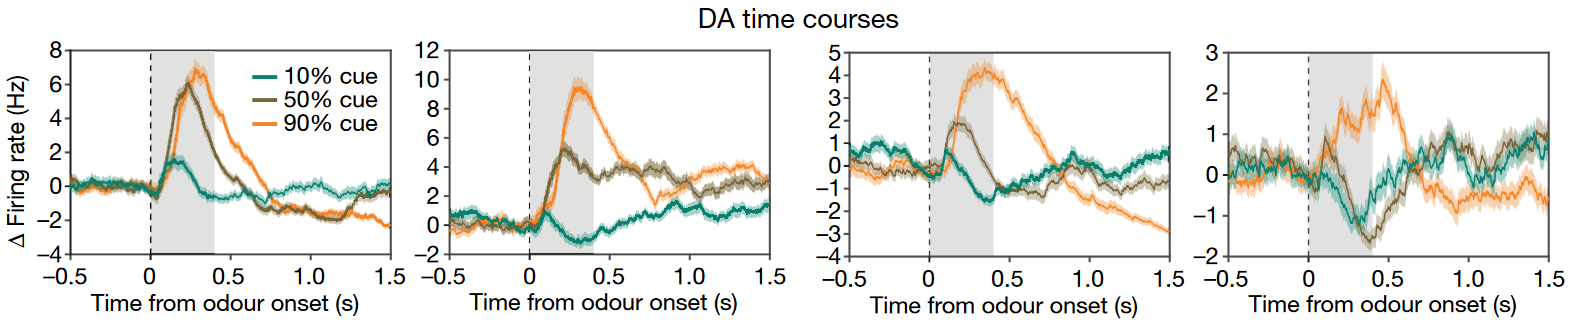
\includegraphics[width=0.8\linewidth]{./img/distr_rl5.png}
        \caption{Activities of four dopaminergic neurons}
    \end{figure}

    An explanation for this behavior of having different reversal points
    is that the weights for positive ($\alpha^+$) and negative ($\alpha^-$) RPEs are different, or, 
    more specifically, the asymmetric scaling factor $\frac{\alpha^+}{\alpha^+ + \alpha^-}$ is different.
    This creates a disequilibrium that can be rebalanced by changing the reversal points of the neurons.
    \begin{figure}[H]
        \centering
        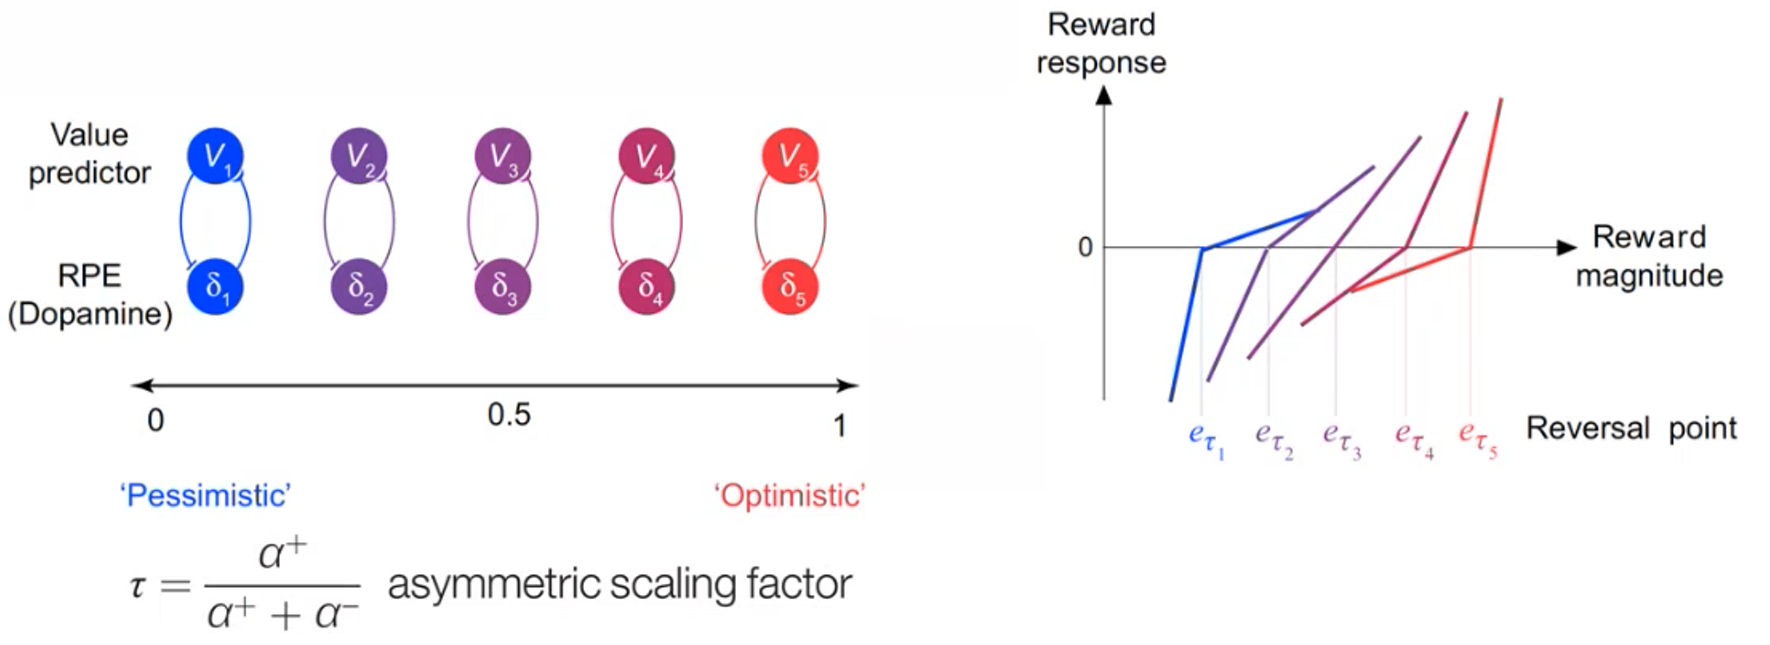
\includegraphics[width=0.65\linewidth]{./img/distr_rl6.png}
    \end{figure}

    Indeed, measurements show that the reversal point and the asymmetric scaling factor are correlated
    indicating the need to shift the reversal point to reach equilibrium.
    \begin{figure}[H]
        \centering
        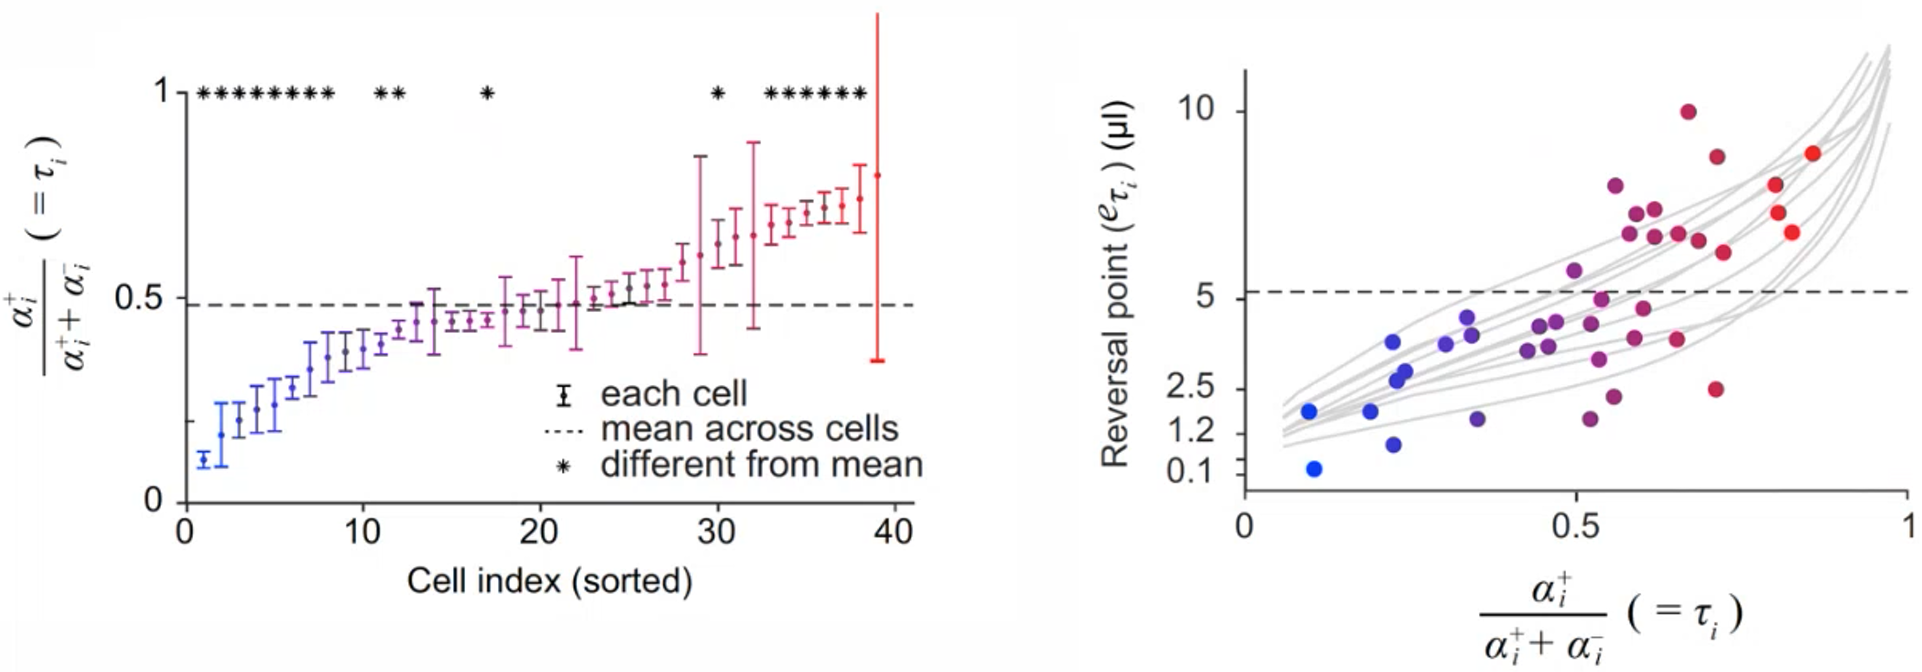
\includegraphics[width=0.65\linewidth]{./img/distr_rl7.png}
    \end{figure}

    By decoding reward distributions from neural responses, it can be seen that:
    \begin{itemize}
        \item Classical RL is not able to predict the correct distribution.
        \item Distributional RL and neuronal data are able to approximate the reward distribution.
    \end{itemize}
    \begin{figure}[H]
        \centering
        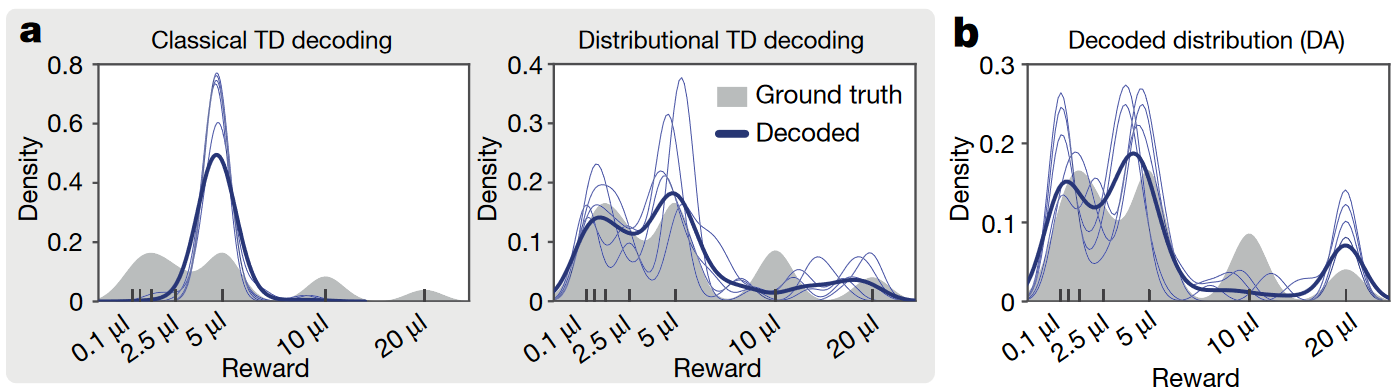
\includegraphics[width=0.7\linewidth]{./img/distr_rl8.png}
    \end{figure}
\end{casestudy}